\subsection{Jacobian 判别法}

设 \(k\) 为环，A 为 \(k\)-代数，J 为 A 的理想，而 \(\bar{d}:\mathrm{J / J^{2}}\to A /\mathrm{J}\otimes_{\mathrm{A}}\Omega_{k}(\mathrm{A})\) 为典范映射。对每个 A/J-代数 R，我们用

\[
\bar {d} _ {\mathrm{R}}: \mathrm{R} \otimes_ {A / \mathrm{J}} \mathrm{J} / \mathrm{J} ^ {2} \longrightarrow \mathrm{R} \otimes_ {\mathrm{A}} \Omega_ {k} (\mathrm{A})
\]

表示由 \(\bar{d}\) 导出的 R-线性映射。若 k-代数 A/J 形式光滑，则 \(\bar{d}\) 具有 A-线性收缩（第 2 节，注 1），并且对每个 R，\(\bar{d}_{R}\) 都具有 R-线性收缩。

更一般地：

引理 3.—— 设 K 为 A 的一个包含 J 的理想。假设存在整数 m，使 \(J \cap K^{m}\) 含于 JK（当 A 为 Noether 环时此条件满足）。若 A/J 关于 K/J-进拓扑在 k 上形式光滑，则映射 \(\bar{d}_{A/K}: A/K \otimes_{A/J} J/J^{2} \longrightarrow A/K \otimes_{A} \Omega_{k}(A)\) 具有 A-线性收缩。

用 C 表示 \(k\)-代数 \(\mathrm{A} / (\mathrm{JK} + \mathrm{K}^m)\)；C 的理想 \(\mathrm{N} = (\mathrm{J} + \mathrm{K}^m) / (\mathrm{JK} + \mathrm{K}^m)\) 平方为零，且商环 C/N 与 \(\mathrm{A} / (\mathrm{J} + \mathrm{K}^m)\) 等同。给 C 与 C/N 赋以离散拓扑，给 A/J 赋以 K/J-进拓扑。典范同态 \(\mathrm{A} / \mathrm{J} \to \mathrm{A} / (\mathrm{J} + \mathrm{K}^m)\) 是连续的；因此它有一个提升 \(\varphi : \mathrm{A} / \mathrm{J} \to \mathrm{A} / (\mathrm{JK} + \mathrm{K}^m)\)。

于是，从 A 到 N 的映射 \(a \mapsto a1_{\mathrm{C}} - \varphi(a1_{\mathrm{A/J}})\) 是一个 \(k\)-导子（\(n^{\circ} 1\)，命题 1），故可写成 \(a \mapsto u(da)\)，其中 \(u \in \mathrm{Hom}_{\mathrm{A}}(\Omega_k(\mathrm{A}), \mathrm{N})\)。但假设 \(\mathrm{J} \cap \mathrm{K}^m \subset \mathrm{JK}\) 蕴含 \(\mathrm{J} \cap (\mathrm{JK} + \mathrm{K}^m) = \mathrm{JK}\)，故典范映射 \(\psi: \mathrm{J/JK} \to \mathrm{N}\) 是双射；因此存在 \(v \in \mathrm{Hom}_{\mathrm{A/K}}(\mathrm{A/K} \otimes_{\mathrm{A}} \Omega_k(\mathrm{A}), \mathrm{J/JK})\)，使得对 A 中的 a，有 \(a1_{\mathrm{C}} = \varphi(a1_{\mathrm{A/J}}) + \psi(v(1 \otimes da))\)。取 a 属于 J，即见 \(v(1 \otimes da)\) 等于 a 在 J/JK 中的类。由于 \(\mathrm{A/K} \otimes_{\mathrm{A/J}} \mathrm{J/J}^2\) 与 J/JK 等同，v 就是所求的收缩。

当代数 A 为 Noether 环时关于 K 的条件成立这一事实，由 III, § 3, 第 1 节，命题 1 的推论 2 可得。

引理 4.—— 假设 A 关于 J-进拓扑在 k 上形式光滑。为使 A/J 在 k 上形式光滑，必须且只须典范映射 \(\bar{d}\) 具有 A-线性收缩。

我们已经知道，若 A/J 在 k 上形式光滑，则映射 \(\bar{d}\) 具有 A-线性收缩（第 2 节，注 1）。反之，假设 \(\bar{d}\) 具有 A-线性收缩。设 \(\pi: A/J^{2} \to A/J\) 为典范满射；由第 1 节的命题 2，存在环同态 \(h: A/J \to A/J^{2}\) 使 \(\pi \circ h = 1_{A/J}\)。设 C 为一个 k-代数，N 为 C 的一个平方为零的理想，\(\rho: C \to C/N\) 为典范满射；给 C 与 C/N 赋以离散拓扑。设 \(u: A/J \to C/N\) 为 k-代数的连续同态。由于 A 关于 J-进拓扑在 k 上形式光滑，存在 k-代数同态 \(v: A \to C\) 使该图表交换

\pandocbounded{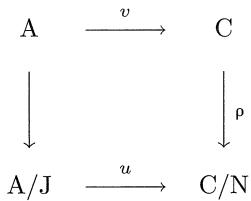
\includegraphics[keepaspectratio]{images/part001_bcdd9d30.jpg}}

其中竖直箭头表示典范满射。我们有 \(v(\mathrm{J})\subset\mathrm{N}\)，从而 \(v(\mathrm{J}^{2})\subset\mathrm{N}^{2}=\{0\}\)，于是 v 通过取商定义了一个同态 \(\bar{v}:\mathrm{A}/\mathrm{J}^{2}\to\mathrm{C}\)，它满足 \(\rho\circ\bar{v}=u\circ\pi\)。那么 \(\bar{v}\circ h\) 是 u 到 C 中的提升。

定理 3.—— 设 \(k\) 为环，A 为形式光滑的 \(k\)-代数，J 为 A 的有限生成理想；令 B=A/J。

\begin{enumerate}
\def\labelenumi{\alph{enumi})}
\tightlist
\item
  设 \(\mathfrak{p}\) 为 B 的素理想，\(\mathfrak{q}\) 为 A 中满足 \(\mathfrak{p}=\mathfrak{q}/J\) 的（素）理想。下列条件等价：
\end{enumerate}

\begin{enumerate}
\def\labelenumi{(\roman{enumi})}
\item
  k-代数 \(B_{\mathfrak{p}}\) 形式光滑；
\item
  存在 \(f\in B-\mathfrak{p}\) 使 k-代数 \(B_{f}\) 形式光滑；
\item
  \(\kappa (\mathfrak{p})\)-线性映射
\end{enumerate}

\[
\bar {d} _ {\kappa (\mathfrak {p})}: \kappa (\mathfrak {p}) \otimes_ {\mathrm{B}} \mathrm{J} / \mathrm{J} ^ {2} \rightarrow \kappa (\mathfrak {p}) \otimes_ {\mathrm{A}} \Omega_ {k} (\mathrm{A})
\]

是单射；

\begin{enumerate}
\def\labelenumi{(\roman{enumi})}
\setcounter{enumi}{3}
\tightlist
\item
  存在整数 \(m \geqslant 0\)、J 的元素 \(f_{1}, \ldots, f_{m}\)（其像 \((f_{1})_{\mathfrak{q}}, \ldots, (f_{m})_{\mathfrak{q}}\) 生成理想 \(J_{\mathfrak{q}}\)），以及 A 的 k-导子 \(D_{1}, \ldots, D_{m}\)，使 \(\det(\mathrm{D}_{j}(f_{i})) \not\in \mathfrak{q}\)。
\end{enumerate}

\begin{enumerate}
\def\labelenumi{\alph{enumi})}
\setcounter{enumi}{1}
\item
  B 中满足 (a) 的诸等价条件的素理想 p 组成的集合在 Spec(B) 中是开集。为使 B 在 k 上形式光滑，必须且只须 B 的每个素（相应地，极大）理想都满足这些条件。
\item
  假设 A 是 Noether 环。(a) 的条件也等价于：
\end{enumerate}

\begin{enumerate}
\def\labelenumi{(\alph{enumi})}
\setcounter{enumi}{21}
\tightlist
\item
  k-代数 \(B_{\mathfrak{p}}\) 关于 \(\mathfrak{p}B_{\mathfrak{p}}\)-进拓扑形式光滑。
\end{enumerate}

此外，在条件 (iv) 之下，理想 \(J_{\mathfrak{q}}\) 是完全割的，且序列 \(((f_{1})_{\mathfrak{q}},\ldots,(f_{m})_{\mathfrak{q}})\) 对 \(A_{\mathfrak{q}}\) 是完全割的。

令 \(M = J/J^{2}\)，\(N = B \otimes_{A} \Omega_{k}(A)\)。B-模 \(M\) 是有限型的，而 B-模 \(N\) 是投射的（\(n^{\circ} 5\)，定理 2 的推论 3）。对每个乘性子集 \(S\)（含于 \(A\)），\(k\)-代数 \(S^{-1}A\) 都形式光滑（\(n^{\circ} 2\)，命题 4, a)）。于是由引理 4，条件 (i) 与 (ii) 分别等价于

(i') 映射 \(\bar{d}_{B_{\mathfrak{p}}}:M_{\mathfrak{p}}\longrightarrow N_{\mathfrak{p}}\) 具有 \(B_{\mathfrak{p}}\)-线性收缩；

(ii') 存在 \(f \in \mathrm{B} - \mathfrak{p}\)，使映射 \(\tilde{d}_{\mathrm{B}_f}: \mathrm{M}_f \to \mathrm{N}_f\) 具有 \(\mathrm{B}_f\)-线性收缩。

把第 8 节的命题 9 应用于环 B 和同态 \(\bar{d}:M\to N\)，即得条件 (i')、(ii'') 与 (iii) 的等价性，并且（再次利用引理 4）也给出 (b) 中的断言。此外，(iii) 等价于：

(iii') 映射 \(\kappa(\mathfrak{q})\otimes_{\mathrm{A}}\mathrm{J}\longrightarrow\kappa(\mathfrak{q})\otimes_{\mathrm{A}}\Omega_{k}(\mathrm{A})\)（由 \(d:\mathrm{J}\to\Omega_{k}(\mathrm{A})\) 导出）是单射，

而 (iv) 可写成：

(iv') 存在整数 \(m\geqslant 0\)、J 的元素 \(f_{1},\ldots,f_{m}\)（其像生成理想 \(J_{\mathfrak{q}}\)，在环 \(A_{\mathfrak{q}}\) 中），以及元素 \(y_{1},\ldots,y_{m}\)（属于 \(\operatorname{Hom}_{\mathrm{A}}(\Omega_{k}(A),A)\)），使 \(\det(\langle y_{j},df_{i}\rangle)\notin\mathfrak{q}\)。

由于 \(\mathrm{A}\)-模 \(\Omega_{k}(A)\) 是投射的（第 5 节，定理 2 的推论 3），把第 8 节的命题 9 应用于环 A 和同态 \(d:\mathrm{J}\to\Omega_{k}(A)\)，即得 (iii') 与 (iv') 的等价性。

最后，假设环 A 是 Noether 环。显然 (i) 蕴含 (v)。在假设 (v) 之下，引理 3 表明映射

\[
\bar {d} _ {\kappa (\mathfrak {q})}: \kappa (\mathfrak {q}) \otimes_ {\mathrm{B} _ {\mathfrak {p}}} \mathrm{J} _ {\mathfrak {q}} / \mathrm{J} _ {\mathfrak {q}} ^ {2} \longrightarrow \kappa (\mathfrak {q}) \otimes_ {\mathrm{A} _ {\mathfrak {q}}} \Omega_ {k} (\mathrm{A} _ {\mathfrak {q}})
\]

是单射，从而得到 (iii)。

在条件 (iv) 之下，我们有 \(m=[\kappa(\mathfrak{q})\otimes_{\mathrm{A}}\mathrm{J}:\kappa(\mathfrak{q})]\)（第 9 节，命题 8）。根据第 5 节的定理 2，理想 \(J_{\mathfrak{q}}\) 是完全割的，且序列 \(((f_1)_{\mathfrak{q}},\ldots,(f_m)_{\mathfrak{q}})\) 对 \(A_{\mathfrak{q}}\) 是完全割的（§ 1, 第 3 节，定理 1 的推论 2）。这就证明了 c)。

推论 1.—— 设 \(k_{0}\) 为环，\(k\) 为 Noether 的形式光滑 \(k_{0}\)-代数，B 为本质有限型的局部 \(k\)-代数。若 \(k_{0}\)-代数 B 关于 \(\mathfrak{m}_{\mathrm{B}}\)-进拓扑形式光滑，则它形式光滑。

存在整数 \(n\geqslant 0\)、\(k[\mathrm{T}_{1},\ldots,\mathrm{T}_{n}]\) 的乘性子集 S，以及一个满的 \(k\)-同态 \(\mathrm{S}^{-1}k[\mathrm{T}_{1},\ldots,\mathrm{T}_{n}]\to\mathrm{B}\)。代数 \(\mathrm{S}^{-1}k[\mathrm{T}_{1},\ldots,\mathrm{T}_{n}]\) 是 Noether 的，且在 k 上形式光滑（第 3 节，例 2 及第 2 节，命题 4, a)），故在 \(k_{0}\) 上也形式光滑（第 2 节，命题 3, a)）。于是推论由定理 3, c) 得出。

推论 2.—— 设 \(k_{0}\) 为环，\(k\) 为 Noether 的形式光滑 \(k_{0}\)-代数，B 为本质有限型的 k-代数。由 B 中使 \(k_{0}\)-代数 \(B_{\mathfrak{p}}\) 形式光滑（关于离散拓扑或 \(\mathfrak{p}B_{\mathfrak{p}}\)-进拓扑）的素理想 p 组成的集合 U 在 Spec(B) 中是开集，且下列条件等价：

\begin{enumerate}
\def\labelenumi{(\roman{enumi})}
\item
  我们有 U = Spec(B)；
\item
  U 包含 B 的所有极大理想；
\item
  \(k_{0}\)-代数 B 形式光滑。
\end{enumerate}

这与前面一样由定理 3 得出。

注 1.—— 当 \(k_{0}\) 是域且我们处于下列两种情形之一时，推论 1 与 2 特别适用：

\begin{enumerate}
\def\labelenumi{\alph{enumi})}
\item
  B 是 \(k_{0}\) 的一个可分扩张上的本质有限型代数（第 3 节，定理 1）；
\item
  B 是 \(k_{0}\)-完备 Noether 局部代数，其剩余域 \(\kappa_{B}\) 是 \(k_{0}\) 的可分扩张（此时我们取 k 为 \(\kappa_{B}\) 上的一个形式幂级数代数，而 B 是它的一个商（第 3 节及 IX, § 3, 第 3 节））。
\end{enumerate}

在上述每种情形中，由推论 2，并考虑到第 7 节的命题 8 以及 § 6 第 4 节的命题 6, b)，可知 \(k_0\)-代数 B 形式光滑当且仅当它绝对正则。

推论 3 (Zariski)。设 \(k\) 为域，A 为正则的 \(k\)-局部代数，J 为 A 的一个不等于 A 的理想。我们假设 \(k\)-代数 A 是本质有限型的或完备的。为使局部环 A/J 正则，必须且只须存在整数 \(m \geqslant 0\)、生成 J 的 J 中元素 \(f_1, \ldots, f_m\)，以及 A 的导子 D \(_1, \ldots, D_m\)，使 det(D \(_j(f_i)\) ) \(\not\in \mathfrak{m}_{\mathrm{A}}\)。此时元素 (f \(_1, \ldots, f_m\) ) 构成 A 的一个坐标系的一部分，且理想 J 是素理想。

设 \(k_0\) 为 \(k\) 的素域。\(k_0\)-代数 A 绝对正则（§ 6, 第 4 节，例 1），故形式光滑（前面的注 1）。基于同样的理由，说 A/J 正则等价于说它是形式光滑的 \(k_0\)-代数。于是第一个断言由定理 3 得出，而定理 3 还蕴含序列 \((f_1,\ldots,f_m)\) 对 A 是完全割的。然后应用 VIII, § 5, 第 3 节的命题 2。

注 2.—— 在推论 3 的假设之下，A-模 \(\Omega(A)\) 是投射的（第 5 节，定理 2 的推论 3），故是自由的；于是 A 到 \(\kappa_{A}\) 中的每个导子都可提升为 A 的导子。因此命题中的条件可表述如下：存在 J 的生成系 \((f_{1},\ldots,f_{m})\) 与导子 \(D_{1},\ldots,D_{m}\)（从 A 到 \(\kappa_{A}\) 中），使 \(\det(D_{j}(f_{i}))\neq0\)。

推论 4 (Zariski)。—— 设 k 为域，A 为本质有限型的 k-代数或完备 Noether 局部环。由 A 中使局部环 A \(_{p}\) 正则的素理想 p 组成的集合在 Spec(A) 中是开集。

只需应用注 1，取 \(k_0\) 为 \(k\) 的素域即可。

\subsection{光滑代数}

引理 5.—— 设 \(\rho: A \to B\) 为 Noether 局部环之间的局部同态。假设 B 在 A 上是本质有限型的。为使 A-代数 B 形式光滑，必须且只须 A-模 B 平坦，且 \(\kappa_{A}\)-代数 \(\kappa_{A} \otimes_{A} B\) 绝对正则。

存在整数 \(n \geqslant 0\)、\(A[T_{1}, \ldots, T_{n}]\) 的素理想 q，以及从 \(A[T_{1}, \ldots, T_{n}]_{q}\) 到 B 的满射同态 h。用 C 表示局部 A-代数 \(A[T_{1}, \ldots, T_{n}]_{q}\)；它是形式光滑的（\(n^{\circ} 3\)，例 2 及 \(n^{\circ} 2\)，命题 4, a)）且在 A 上平坦，并且可把 B 等同于 A-代数 C/J，其中 \(J = \text{Ker}(h)\)。

令 \(\overline{\mathrm{C}} = \kappa_{\mathrm{A}} \otimes_{\mathrm{A}} \mathrm{C}\)，\(\overline{\mathrm{B}} = \kappa_{\mathrm{A}} \otimes_{\mathrm{A}} \mathrm{B}\)。假设 B 在 A 上形式光滑。于是 \(\kappa_{\mathrm{A}}\)-代数 \(\overline{\mathrm{B}}\) 形式光滑（第 2 节，命题 4, b)），故绝对正则（第 5 节，定理 2 的推论 2）。此外，由于 \(\overline{\mathrm{C}} / \overline{\mathrm{JC}}\) 与 \(\overline{\mathrm{B}}\) 等同，且 \(\kappa_{\mathrm{A}}\)-代数 \(\overline{\mathrm{C}}\) 形式光滑，故理想 \(\overline{\mathrm{JC}}\)（在 \(\overline{\mathrm{C}}\) 中）是完全割的（第 5 节，定理 2）。于是由 § 5, 第 6 节，命题 6 可知 A-模 B 平坦。

反之，假设 B 在 A 上平坦，且 \(\kappa_{\mathrm{A}}\)-代数 \(\overline{\mathbf{B}}\) 绝对正则。于是 \(\kappa_{\mathrm{A}}\)-局部代数 \(\overline{\mathbf{B}}\) 形式光滑（第 9 节的注 1，取 \(k = k_0 = \kappa_{\mathrm{A}}\)）。令 \(\overline{\mathbf{J}} = \kappa_{\mathrm{A}} \otimes_{\mathrm{A}} \mathrm{J}\)；由于 B 是平坦 A-模，典范映射 \(\overline{\mathbf{J}} \to \overline{\mathbf{J}}\overline{\mathbf{C}}\) 是双射，且 \(\overline{\mathbf{B}}\) 与 \(\overline{\mathbf{C}}/\overline{\mathbf{J}}\) 等同。由此（第 2 节的注 1）可知典范映射

\[
\overline {{\mathrm{J}}} / \overline {{\mathrm{J}}} ^ {2} \longrightarrow \overline {{\mathrm{B}}} \otimes_ {\overline {{\mathrm{C}}}} \Omega_ {\kappa_ {\mathrm{A}}} (\overline {{\mathrm{C}}})
\]

是单射且具有一个收缩。而 \(\overline{\mathrm{J}}/\overline{\mathrm{J}}^{2}\) 与 \(\kappa_{\mathrm{A}}\otimes_{\mathrm{A}}\mathrm{J}/\mathrm{J}^{2}\) 等同，故与 \(\overline{\mathrm{B}}\otimes_{\mathrm{B}}\mathrm{J}/\mathrm{J}^{2}\) 等同。另一方面，\(\overline{\mathrm{C}}\)-模 \(\Omega_{\kappa_{\mathrm{A}}}(\overline{\mathrm{C}})\) 典范地同构于 \(\overline{\mathrm{C}}\otimes_{\mathrm{C}}\Omega_{\mathrm{A}}(\mathrm{C})\)（A, III, 第 136 页，命题 20），故 \(\overline{\mathrm{B}}\otimes_{\overline{\mathrm{C}}}\Omega_{\kappa_{\mathrm{A}}}(\overline{\mathrm{C}})\) 典范地同构于 \(\overline{\mathrm{B}}\otimes_{\mathrm{C}}\Omega_{\mathrm{A}}(\mathrm{C})\)。对 \(\overline{\mathrm{B}}\) 的极大理想取商，即得一个单同态

\[
\kappa_ {B} \otimes_ {B} J / J ^ {2} \longrightarrow \kappa_ {B} \otimes_ {C} \Omega_ {A} (C)
\]

它正是 \(\bar{d}_{\kappa_{\mathrm{B}}}\)。于是 B 在 A 上形式光滑（定理 3）。

定理 4.—— 设 A 为 Noether 环，B 为本质有限型的 A-代数。下列条件等价：

\begin{enumerate}
\def\labelenumi{(\roman{enumi})}
\item
  A-代数 B 形式光滑；
\item
  对每个 \(\mathfrak{q} \in \operatorname{Spec}(\mathrm{B})\)，A-代数 \(\mathrm{B}_{\mathfrak{q}}\) 形式光滑（相应地，关于 \(\mathfrak{q}\mathrm{B}_{\mathfrak{q}}\)-进拓扑形式光滑）；
\item
  A-模 B 平坦，且对每个 \(\mathfrak{p} \in \operatorname{Spec}(A)\)，\(\kappa(\mathfrak{p})\)-代数 \(\kappa(\mathfrak{p}) \otimes_{A} B\) 绝对正则；
\item
  A-模 B 平坦，且对每个正则 A-代数 R，环 R ⊗\_A B 正则；
\item
  A-模 B 平坦，且同态 \(\mu:B\otimes_{A}B\to B\)（由 \(\mu(x\otimes y)=xy\) 定义）的核是完全割理想。
\end{enumerate}

(i) 与 (ii) 的等价性由第 9 节定理 3 的推论 2 得出。

(i)⇒(v)：假设 A-代数 B 形式光滑。设 q 为 B 的素理想，p 为它在 A 中的原像。\(A_{\mathfrak{p}}\)-代数 \(B_{\mathfrak{q}}\) 形式光滑（第 2 节的命题 4, a)），故平坦（引理 5）；因而 A-模 B 平坦（II, § 3, 第 4 节，命题 15）。另一方面，环 B ⊗A B 是 Noether 的（§ 6, 第 1 节，命题 2 的推论），故由第 5 节定理 2 的推论 3，理想 Ker μ 是完全割的。

(v)⇒(iii)：假设条件 (v) 满足。令 I = Ker(μ)。设 p ∈ Spec(A)。映射

\[
1 \otimes \mu : \kappa (\mathfrak {p}) \otimes_ {\mathrm{A}} (\mathrm{B} \otimes_ {\mathrm{A}} \mathrm{B}) \rightarrow \kappa (\mathfrak {p}) \otimes_ {\mathrm{A}} \mathrm{B}
\]

等同于映射

\[
\mu_ {\mathfrak {p}}: (\kappa (\mathfrak {p}) \otimes_ {\mathrm{A}} \mathrm{B}) \otimes_ {\kappa (\mathfrak {p})} (\kappa (\mathfrak {p}) \otimes_ {\mathrm{A}} \mathrm{B}) \rightarrow \kappa (\mathfrak {p}) \otimes_ {\mathrm{A}} \mathrm{B}
\]

它是由 \(\kappa(\mathfrak{p})\)-代数 \(\kappa(\mathfrak{p})\otimes_{\mathrm{A}}\mathrm{B}\) 的乘法导出的。理想 \(\operatorname{Ker}(\mu_{\mathfrak{p}})\) 与 \(\mathrm{I}(\kappa(\mathfrak{p})\otimes_{\mathrm{A}}(\mathrm{B}\otimes_{\mathrm{A}}\mathrm{B}))\) 等同。由于 A-模 B 平坦（\(\S 5\), 第 6 节，命题 6），它是完全割的。于是断言 (iii) 由 \(\S 6\) 第 5 节的命题 8 得出。

(iii)⇒(ii)：设 q 为 B 的素理想，p 为其在 A 中的原像。在 (iii) 的假设之下，A \(_{p}\)-模 B \(_{q}\) 平坦，而 κ(p)-代数 κ(p) ⊗A \(_{p}\) B \(_{q}\)（它与 κ(p) ⊗A B 的一个分式环等同）绝对正则（§ 6, 第 4 节，命题 6）。于是由引理 5，B \(_{q}\) 在 A \(_{p}\) 上形式光滑，故在 A 上形式光滑（第 2 节，命题 3 与 4）。

(iii)⇒(iv)：设在 (iii) 的假设之下。设 R 为正则 A-代数。R-模 R ⊗A B 平坦（I, § 2, 第 7 节，命题 8 的推论 2）。设 r 为 R 的素理想，p 为其在 A 中的原像；环 κ(r)⊗R(R⊗AB)（它与 κ(r)⊗κ(p) (κ(p)⊗A B) 等同）是正则的（§ 6, 第 4 节，命题 7 的推论 2）。于是环 R ⊗A B 正则（§ 4, 第 5 节，命题 9 的推论）。

(iv)⇒ (iii)：设 p 为 A 的素理想，k 为 κ(p) 的一个扩张；在 (iv) 的假设之下，环 \(k \otimes_{\kappa(\mathfrak{p})} (\kappa(\mathfrak{p}) \otimes_{\mathrm{A}} \mathrm{B})\)（它与 \(k \otimes_{A} B\) 等同）是正则的，由此得 (iii)。

定义 2.—— 设 A 为 Noether 环。若 A-代数 B 是本质有限型的且满足定理 4 的诸等价条件，则称它是光滑的。

命题 10.—— 设 A 为 Noether 环。

\begin{enumerate}
\def\labelenumi{\alph{enumi})}
\item
  设 A' 为 Noether A-代数，B 为光滑 A-代数。则 A'-代数 A' ⊗\_A B 光滑。
\item
  设 B 为光滑 A-代数，C 为光滑 B-代数。则 A-代数 C 光滑。
\item
  设 B 与 C 为两个光滑 A-代数。则 A-代数 B ⊗A C 光滑。
\end{enumerate}

这由第 2 节的命题 4 以及关于本质有限型代数的类似命题（§ 6, 第 1 节）得出。

例.—— 1) 域 \(k\) 上的光滑代数恰是本质有限型且绝对正则的 \(k\)-代数。

\begin{enumerate}
\def\labelenumi{\arabic{enumi})}
\setcounter{enumi}{1}
\tightlist
\item
  设 A 为 Noether 环，\(\mathbf{T} = (\mathrm{T}_i)_{i\in I}\) 为有限的未定元族。A-代数 A{[}T{]} 是光滑的。更一般地，设 \(\mathrm{F}_1,\ldots ,\mathrm{F}_m\) 为 A{[}T{]} 的元素，B 为 A-代数 A{[}T{]}/ \((\mathrm{F}_1,\dots ,\mathrm{F}_m)\)。若在 B 的每个极大理想 \(\mathfrak{n}\) 处，模 \(\mathfrak{n}\) 之下矩阵 \(\left(\frac{\partial\mathrm{F}_j}{\partial\mathrm{T}_i}\right)\) 的类都有秩 \(m\)，则 A-代数 B 光滑（第 9 节，定理 3）。
\end{enumerate}

\section{有限长度模的对偶性}

\subsection{不可分解内射模}

设 A 为环。关系「I 是不可分解内射 A-模的一个类」是集化关系（A, X, 第 21 页，推论 1）；我们将用 \(\mathcal{I}(A)\) 表示不可分解内射 A-模的诸类所成的集合。

命题 1.—— 设 A 为 Noether 环。对 A 的每个素理想 p，设 \(e_{\mathfrak{p}}: \mathrm{A}/\mathfrak{p} \to \mathrm{I}(\mathfrak{p})\) 为 \(\mathrm{A}/\mathfrak{p}\) 的一个内射包（A, X, § 1, 第 9 节）。

\begin{enumerate}
\def\labelenumi{\alph{enumi})}
\item
  A-模 I(p) 都是不可分解的。
\item
  设 I 为不可分解内射 A-模；集合 Ass(I) 只含一个元素。
\item
  映射 \(\mathfrak{p} \mapsto \operatorname{cl}(\operatorname{I}(\mathfrak{p}))\) 是从 \(\operatorname{Spec}(\operatorname{A})\) 到 \(\mathcal{I}(A)\) 上的双射。其逆双射把 \(\mathcal{I}(\operatorname{A})\) 的元素 I 对应到 \(\operatorname{Ass}(\operatorname{I})\) 的唯一元素。
\end{enumerate}

设 \(\mathfrak{p} \in \operatorname{Spec}(A)\)；我们来证明模 \(I(\mathfrak{p})\) 不可分解。由 A, X, 第 21 页，推论 2，只需证明：若 \(\mathfrak{a}\) 与 \(\mathfrak{b}\) 是 A 的包含 \(\mathfrak{p}\) 且不等于 \(\mathfrak{p}\) 的理想，则理想 \(\mathfrak{a} \cap \mathfrak{b}\) 不等于 \(\mathfrak{p}\)；或者，若 \(a\) 是 \(\mathfrak{a} - \mathfrak{p}\) 的元素而 \(b\) 是 \(\mathfrak{b} - \mathfrak{p}\) 的元素，则乘积 \(ab\) 属于 \((\mathfrak{a} \cap \mathfrak{b}) - \mathfrak{p}\)。

设 I 为不可分解内射 A-模，p、q 为 Ass(I) 的元素。于是 I 包含一个同构于 A/p 的子模 M 和一个同构于 A/q 的子模 N。我们有 M ∩ N ≠ 0（A, X, 第 21 页，命题 14）；对 M ∩ N 的每个非零元素 x，有 p = Ann x = q。由于 Ass(I) 非空（IV, § 1, 第 1 节，命题 2 的推论 1），它只含一个元素 p(I)。

这样我们定义了两个映射：\(\mathfrak{p} \mapsto \operatorname{cl}(I(\mathfrak{p}))\)（从 \(\operatorname{Spec}(A)\) 到 \(\mathcal{I}(A)\)）与 \(I \mapsto \mathfrak{p}(I)\)（从 \(\mathcal{I}(A)\) 到 \(\operatorname{Spec}(A)\)）；我们来证明这两个映射互为逆双射。设 \(\mathfrak{p} \in \operatorname{Spec}(A)\)；则 \(\mathfrak{p}\) 属于 \(\operatorname{Ass}(I(\mathfrak{p}))\)，因而是 \(\operatorname{Ass}(I(\mathfrak{p}))\) 的唯一元素。设 \(I\) 为不可分解内射 A-模，而 \(\mathfrak{p}\) 为 \(\operatorname{Ass}(I)\) 的唯一元素；则 \(I\) 是 \(A/\mathfrak{p}\) 的一个内射包（A, X, 第 21 页，命题 14）。命题证毕。

注 1.——设 I 为不可分解内射 A-模，p 为 Ass(I) 的唯一元素；由命题 1，I 包含一个同构于 A/p 的子模，且 I 是它的内射包。一般而言这样的子模并不唯一，取 A = Z、p = 0、I = Q 即见。

对 \(\mathfrak{p}\)（\(\mathrm{A}\) 中的素理想）的每一个，如上选取 \((\mathrm{I}(\mathfrak{p}), e_{\mathfrak{p}})\) 作为 \(\Lambda/\mathfrak{p}\) 的内射包。由 \(\mathrm{A}\), X, 第 22 页，定理 3，我们有：

定理 1.—— 设 A 为 Noether 环。对每个内射 A-模 I，存在唯一的基数族 \((a_{\mathfrak{p}})_{\mathfrak{p}\in\operatorname{Spec}(\mathrm{A})}\)，使 I 同构于 \(\bigoplus_{\mathfrak{p}}\mathrm{I}(\mathfrak{p})^{(a_{\mathfrak{p}})}\)。

由 IV, § 1, 第 1 节，命题 3 的推论 1，集合 Ass(I) 是族 \((a_{\mathfrak{p}})\) 的支撑集。

注 2. 设 \(A\) 为 Noether 环，M 为 A-模，\(e: \mathrm{M} \to \mathrm{I}\) 为 M 的一个内射包。集合 Ass(M) 等于 Ass(I)：事实上，包含关系 Ass(M) ⊂ Ass(I) 是显然的。另一方面，若 \(\mathfrak{p}\) 是 Ass(I) 的元素，则 I 包含一个同构于 \(A/\mathfrak{p}\) 的子模 N；由于 \(A\)-模 \(e^{-1}(\mathrm{N})\) 非零，我们有 \(\operatorname{Ass}(e^{-1}(\mathrm{N})) = \{\mathfrak{p}\}\)。这证明 \(\mathfrak{p}\) 与 \(e^{-1}(\mathrm{N})\) 相伴，从而与 M 相伴，断言得证。

采用定理中的记号，并进而假设 Ass(M) 有限。对每个 \(\mathfrak{q} \in \operatorname{Ass}(M)\)，用 \(Q_{\mathfrak{q}}\) 表示 \(\bigoplus_{\mathfrak{p} \in \operatorname{Ass}(M) - \{\mathfrak{q}\}} I(\mathfrak{p})^{(a_{\mathfrak{p}})}\) 与 M 的交。则 \((Q_{\mathfrak{q}})_{\mathfrak{q} \in \operatorname{Ass}(M)}\) 是 M 中零子模的一个既约准素分解（IV, § 2, 第 3 节，定义 3）。事实上，我们有 \(\cap Q_{\mathfrak{q}} = 0\)；由于 \(M/Q_{\mathfrak{q}}\) 等同于 \(I(\mathfrak{q})^{(a_{\mathfrak{q}})}\) 的一个非零子模，有 \(\operatorname{Ass}(M/Q_{\mathfrak{q}}) = \{\mathfrak{q}\}\)，于是只需应用同处的命题 4。

例.—— 设 A 为主理想环，K 为其分式域。内射 A-模就是可除 A-模（A, X, 第 17 页，推论 2）。A-模 K 是 A 的一个内射包（A, X, 第 20 页，例 1）。设 \(p\) 为 A 的极端元，\(\mathfrak{p}\) 为（极大）理想 \(Ap\)。用 \(e: A/\mathfrak{p} \longrightarrow K/A_{\mathfrak{p}}\) 表示把元素 \(a \in A\) 的类映到 \(a/p\) 的类的同态。我们来证明 \((K/A_{\mathfrak{p}}, e)\) 是 \(A/\mathfrak{p}\) 的一个内射包。同态 \(e\) 是单射。A-模 \(K/A_{\mathfrak{p}}\) 是可除模的一个商，故可除。设 \(x\) 为 \(K/A_{\mathfrak{p}}\) 的一个非零元素；它是元素 \(a/p^n\)（属于 K）的类，其中 \(a \in A - \{0\}\) 且 \(n \geqslant 1\)（A, VII, 第 10 页，定理 2）。于是我们有 \(p^{n-1}x = e(a)\)，从而 \(e(Ax) \neq 0\)，这就证明了我们的断言。

于是由定理 1，每个可除 A-模都是若干同构于 K 或 \(K/A_{p}\)（p 为 A 的某个极大（主）理想）的 A-模的直和。

\subsection{不可分解内射模的结构}

引理 1.—— 设 A 为环，a 为 A 的理想，I 为 A-模。对每个整数 \(n \geqslant 0\)，用 \(I_{n}\) 表示 I 中被 \(a^{n}\) 零化的元素组成的子模。

\begin{enumerate}
\def\labelenumi{\alph{enumi})}
\item
  假设 A-模 I 是内射的。则 \(\mathrm{A} / \mathfrak{a}^n\)-模 \(\mathrm{I}_n\) 对每个 \(n \geqslant 0\) 都是内射的。
\item
  假设环 A 是 Noether 的，且对每个 \(n \geqslant 0\)，\(\mathrm{A} / \mathfrak{a}^n\)-模 \(\mathrm{I}_n\) 都是内射的。则诸 \(\mathrm{I}_n\) 的并是一个内射 A-模。
\item
  \(\mathbf{A} / \mathfrak{a}^n\)-模 \(\mathrm{I}_n\) 同构于 \(\operatorname{Hom}_{\mathbf{A}}(\mathbf{A} / \mathfrak{a}^n, \mathbf{I})\)，后者是内射的（A, X, 第 18 页，命题 11）。
\item
  设 J 为诸 \(I_{n}\) 之并，b 为 A 的理想，\(f : b \to J\) 为一个 A-同态。剩下要证（A, X, 第 16 页，命题 10）的是：存在 J 的元素 x，使对每个 \(f(b) = bx\) 有 \(b \in b\)。由于 b 是有限生成的，存在整数 n，使 \(f(\mathfrak{b}) \subset \mathrm{I}_{n}\)，即 \(f(\mathfrak{a}^{n}\mathfrak{b}) = 0\)。根据 III, § 3, 第 1 节，命题 1 的推论 2，存在整数 \(m \geqslant n\) 使 \(a^{m} \cap b \subset a^{n}b\)，从而 \(f(\mathfrak{a}^{m} \cap \mathfrak{b}) = 0\)。于是 f 诱导出一个 A/\(a^{m}\)-线性同态，从 \(\mathfrak{b}/(\mathfrak{a}^{m} \cap \mathfrak{b})\) 到 \(I_{m}\)；由于 A/ \(a^{m}\)-模 \(I_{m}\) 是内射的，存在 \(I_{m}\) 的元素 x，使对每个 \(f(b) = bx\) 有 \(b \in b\)，由此得 b)。
\end{enumerate}

设 \(\mathfrak{a}\) 为 A 的理想；以下我们约定 \(\mathfrak{a}^n = \mathrm{A}\)（对每个整数 \(n \leqslant 0\)）。设 E 为 A-模。对每个 \(n \in \mathbf{Z}\)，用 \(\mathrm{E}_n\) 表示 E 中被 \(\mathfrak{a}^n\) 零化的元素组成的子模；设 \(\mathrm{gr}^{\mathfrak{a}}(\mathrm{E})\) 为 \(\mathbf{Z}\) 型分次 A-模，使得对每个整数 \(\mathrm{gr}^{\mathfrak{a}}(\mathrm{E})_m = \mathrm{E}_{-m+1}/\mathrm{E}_{-m}\) 有 \(m\)。模 \(\mathrm{gr}^{\mathfrak{a}}(\mathrm{E})_m\) 在 \(m \geqslant 1\) 时为零，而 \(\mathrm{gr}^{\mathfrak{a}}(\mathrm{E})_0\) 等同于 \(\mathrm{E}_1\)。设 \(\mathrm{gr}(\mathrm{A})\) 为 A 关于 \(\mathfrak{a}\)-进滤过的伴随分次环：对每个 \(\mathrm{gr}(\mathrm{A})_n = \mathfrak{a}^n/\mathfrak{a}^{n+1}\) 我们有 \(n \in \mathbf{Z}\)。设 \(n\) 与 \(m\) 为整数。对双线性映射 \((a,x) \mapsto ax\)（从 \(\mathfrak{a}^n \times \mathrm{E}_{-m+1}\) 到 \(\mathrm{E}_{-m-n+1}\)）取商，我们导出一个 A/ \(\mathfrak{a}\)-双线性映射

\[
\alpha_ {n, m}: \mathrm{gr} (\mathrm{A}) _ {n} \times \mathrm{gr} ^ {\mathfrak {a}} (\mathrm{E}) _ {m} \longrightarrow \mathrm{gr} ^ {\mathfrak {a}} (\mathrm{E}) _ {n + m},\tag{1}
\]

它在 gr \(^{a}\) (E) 上定义了一个分次 gr(A)-模结构。对每个 \(n \in \mathbf{Z}\)，由 A/a-双线性映射 \(\alpha_{n,-n} : \text{gr}(A)_n \times \text{gr}^{a}(E)_{-n} \longrightarrow E_1\) 导出一个 A/a-线性映射 \(\beta_{E,n} : \text{gr}^{a}(E)_{-n} \longrightarrow \text{Hom}_{A/\alpha}(\text{gr}(A)_n, E_1)\)；诸映射 \(\beta_{E,n}\) 是一个分次 A/a-模同态的各分量，该同态称为典范同态。

\[
\beta_ {\mathrm{E}}: \operatorname{gr} ^ {a} (\mathrm{E}) \longrightarrow \operatorname{Homgr} _ {\mathrm{A} / \mathfrak{a}} (\operatorname{gr} (\mathrm{A}), \mathrm{E} _ {1}).\tag{2}
\]

对 \(a \in \text{gr(A)}\)、\(x \in \text{gr}^{\mathfrak{a}}(\text{E})\)，\(\beta_{\text{E}}(x)(a)\) 按定义是 \(\text{gr}^{\mathfrak{a}}(\text{E})_0 = \text{E}_1\) 中元素 \(ax\)（属于 \(\text{gr}^{\mathfrak{a}}(\text{E})\)）的分量。由此可知，\(\beta_{\text{E}}\) 是 \(\text{gr(A)}\)-线性的，只要给 \(\text{Homgr}_{\text{A}/\mathfrak{a}}(\text{gr(A)}, \text{E}_1)\) 赋以由公式 \(\text{gr(A)}\)（其中 \((bf)(a) = f(ab)\) 属于 \(a, b\)，\(\text{gr(A)}\) 属于 \(f\)）所定义的 \(\text{Homgr}_{\text{A}/\mathfrak{a}}(\text{gr(A)}, \text{E}_1)\)-模结构。

命题 2.—— 设 A 为 Noether 环，a 为 A 的理想，E 为 A-模，M 为 E 的被 a 零化的子 A-模。下列条件等价：

\begin{enumerate}
\def\labelenumi{(\roman{enumi})}
\item
  E 是 M 的一个内射包；
\item
  \(\mathrm{A}/\mathfrak{a}\)-模 \(\mathrm{E}_1\) 是 \(\mathrm{A}/\mathfrak{a}\)-模 \(\mathrm{M}\) 的内射包；模 \(\mathrm{E}\) 是诸 \(\mathrm{E}_n\) 的并，且典范映射 \(\beta_{\mathrm{E}}\) 是双射。
\end{enumerate}

假设条件 (i) 满足。A/a-模 \(E_{1}\) 是内射的（引理 1, a)），且包含 M；由于 \(A/a\) 的每个含于 \(E_{1}\) 的子模都是 E 的子 A-模，故 \(E_{1}\) 是 A/a-模 M 的一个内射包。由引理 1，诸 \(E_{n}\) 之并是 E 的一个包含 M 的内射子 A-模，故等于 E。由于 E 内射，对所有 \(n \geqslant 0\) 有正合列

\[
0 \to \operatorname{Hom} _ {\mathrm{A}} (\mathrm{A} / \mathfrak {a} ^ {n}, \mathrm{E}) \longrightarrow \operatorname{Hom} _ {\mathrm{A}} (\mathrm{A} / \mathfrak {a} ^ {n + 1}, \mathrm{E}) \longrightarrow \operatorname{Hom} _ {\mathrm{A}} (\mathfrak {a} ^ {n} / \mathfrak {a} ^ {n + 1}, \mathrm{E}) \to 0;
\]

由于 \(\mathrm{Hom}_{\mathrm{A}}(\mathrm{A}/\mathfrak{a}^{m},\mathrm{E})\) 等同于 \(\mathrm{E}_{m}\)（对每个 \(m\)），且从 \(\mathrm{Hom}_{\mathrm{A}}(\mathfrak{a}^{n}/\mathfrak{a}^{n+1},\mathrm{E}_{1})\) 到 \(\mathrm{Hom}_{\mathrm{A}}(\mathfrak{a}^{n}/\mathfrak{a}^{n+1},\mathrm{E})\) 的典范单射是双射，我们推出典范同态 \(\beta_{\mathrm{E}}\) 是双射，由此得 (ii)。

假设 (ii) 满足。设 \(e: \mathrm{M} \to \mathrm{I}\) 为 M 的一个内射包。由于 I 内射，存在 A-线性映射 \(\varphi: \mathrm{E} \to \mathrm{I}\) 延拓 \(e\)。而 \(\varphi\) 把 \(\mathrm{E}_n\) 映到 \(\mathrm{I}_n\) 中（对每个 \(n\)），从而诱导出同态 \(\mathrm{gr}^{\mathfrak{a}}(\varphi):\mathrm{gr}^{\mathfrak{a}}(\mathrm{E})\to \mathrm{gr}^{\mathfrak{a}}(\mathrm{I})\) 与 \(\varphi_{1}:\mathrm{E}_{1}\rightarrow \mathrm{I}_{1}\)，并使下图交换

\[
\begin{array}{c c c} \operatorname{gr} ^ {\mathfrak {a}} (\mathrm{E}) & \xrightarrow {\beta_ {\mathrm{E}}} & \operatorname{Homgr} _ {\mathrm{A} / \mathfrak {a}} (\operatorname{gr} (\mathrm{A}), \mathrm{E} _ {1}) \\ \operatorname{gr} ^ {\mathfrak {a}} (\varphi) \Bigg \downarrow & & \Bigg \downarrow \operatorname{Homgr} (1, \varphi_ {1}) \\ \operatorname{gr} ^ {\mathfrak {a}} (\mathrm{I}) & \xrightarrow {\beta_ {\mathrm{I}}} & \operatorname{Homgr} _ {\mathrm{A} / \mathfrak {a}} (\operatorname{gr} (\mathrm{A}), \mathrm{I} _ {1}). \end{array}
\]

由于 \(E_{1}\) 与 \(I_{1}\) 都是 A/a-模 M 的内射包，同态 \(\varphi_{1}\) 是双射；由于 \(\beta_{E}\) 与 \(\beta_{I}\) 都是双射，可知 \(\mathrm{gr}^{\mathfrak{a}}(\varphi)\) 是双射。由对 n 的归纳法，这蕴含 \(\varphi\) 诱导一个从 \(E_{n}\) 到 \(I_{n}\) 上的双射（对每个 \(n \geqslant 1\)）；因此 \(\varphi\) 是双射，由此得 (i)。

引理 2.—— 设 A 为环，a 为 A 的有限生成理想，M 为每个元素都被 a 的某个幂零化的 A-模。用 A-hat 表示 A 关于 a-进拓扑的分离完备化。

\begin{enumerate}
\def\labelenumi{\alph{enumi})}
\item
  在 M 上存在唯一的 \(\widehat{\mathrm{A}}\) -模结构，它延拓给定的 A-模结构。
\item
  M 的子 A-hat-模即其子 A-模，并且 Hom \(_{\text{A}}\) (M, P) = Hom \(_{\widehat{\text{A}}}\) (M, P) 对每个 \(\widehat{\text{A}}\) -模 P 成立。
\item
  把 \(\widehat{\mathbf{A}}\) 等同于环 \(\mathrm{A} / \mathfrak{a}^n\) 的逆极限，并给 M 赋以离散拓扑。设 \(a = (a_n)\) 为 \(\widehat{\mathbf{A}}\) 的一个元素，并设 \(x\) 为 M 的一个元素。由于 \(x\) 被 \(\mathfrak{a}\) 的某个幂零化，序列 \((a_n x)\) 平稳；用 \(ax\) 表示它的极限。映射 \((a, x) \mapsto ax\) 在 M 上定义了一个 \(\widehat{\mathbf{A}}\) -模结构，它延拓给定的 A-模结构。
\end{enumerate}

反之，设 M 上给定这样一个结构；设 \(a = (a_{n})\) 为 \(\widehat{\mathrm{A}}\) 的元素，\(x\) 为 M 的元素，\(m\) 为使 \(\mathfrak{a}^{m}x = 0\) 成立的整数。对每个整数 \(n\)，\(a - a_{n}\) 属于 \(\widehat{\mathfrak{a}^{n}}\)，后者等于 \(\mathfrak{a}^{n}\widehat{\mathrm{A}}\)（III, § 2, 第 12 节，命题 16 的推论 2）；因而等式 \(ax = a_{n}x\) 对 \(n \geqslant m\) 成立，由此得唯一性断言。

\begin{enumerate}
\def\labelenumi{\alph{enumi})}
\setcounter{enumi}{1}
\tightlist
\item
  由前所述，等式 \(Ax = \widehat{A}x\) 对每个 \(x \in M\) 都成立；于是子 \(\widehat{A}\)-模（在 \(M\) 中）就是它的子 \(A\)-模。最后，设 \(u\) 为一个 \(A\)-线性同态，它把 \(M\) 映入一个 \(\widehat{A}\)-模 \(P\)。设 \(a = (a_n)\) 为 \(\widehat{A}\) 的元素，\(x\) 为 \(M\) 的元素，\(m\) 为使 \(\mathfrak{a}^m x = 0\) 成立的整数；则有 \(\mathfrak{a}^m u(x) = 0\)。由于 \(a - a_m\) 属于 \(\mathfrak{a}^m\widehat{A}\)，有
\end{enumerate}

\[
u (a x) = u \left(a _ {m} x\right) = a _ {m} u (x) = a u (x),
\]

因此 u 是 A-hat-线性的。

命题 3.—— 设 A 为 Noether 环，p 为 A 的素理想，e : A/p → I 为 A-模 A/p 的一个内射包。对每个整数 n ≥ 0，用 I \(_{n}\) 表示 I 中被 p \(^{n}\) 零化的元素组成的子模。

\begin{enumerate}
\def\labelenumi{\alph{enumi})}
\item
  A-模 I 是诸 \(I_{n}\) 的并。单射 \(\Lambda/p \to I_{1}\) 延拓为一个从 \(\kappa(\mathfrak{p})\) 到 \(I_{1}\) 上的同构；用这个同构把 \(\kappa(\mathfrak{p})\) 与 \(I_{1}\) 等同。对每个整数 \(n \geqslant 0\)，\(\Lambda/p\)-模结构在 \(I_{n+1}/I_{n}\) 上经由纯量限制得自唯一的 \(\kappa(\mathfrak{p})\)-向量空间结构；典范同态 \(\beta_{I,-n}: I_{n+1}/I_{n} \longrightarrow \operatorname{Hom}_{\mathrm{A}/\mathfrak{p}}(\mathfrak{p}^{n}/\mathfrak{p}^{n+1}, \kappa(\mathfrak{p}))\) 是 \(\kappa(\mathfrak{p})\)-向量空间之间的同构，维数有限。
\item
  在 I 上存在唯一的 \(\mathrm{A_p}\) -模结构，它诱导出 I 的 A-模结构。典范同态 \(\widehat{\mathrm{A_p}} \longrightarrow \mathrm{End}_{\mathrm{A}}(\mathrm{I})\) 是双射。
\end{enumerate}

由 A, X, 第 20 页，例 1，A/p-模 \(\kappa(\mathfrak{p})\) 是 A/p 的一个内射包。于是由命题 2，I \(_1\) 等同于 \(\kappa(\mathfrak{p})\)，I 是诸 I \(_m\) 的并，且对每个整数 \(n \geqslant 0\)，\(\beta_{1,-n}\) 是 A/p-模的同构。对 A/p 的每个非零元素 \(a\)，以 \(a\) 为比的乘法映射在 Hom \(_{\text{A/p}}(\mathfrak{p}^n/\mathfrak{p}^{n+1}, \kappa(\mathfrak{p}))\) 中可逆，因而在 I \(_{n+1}\) /I \(_n\) 中也可逆，这就证明了 a)。

设 \(s \in A - p\)。由于乘法映射 \(s_{A/p}\) 是单射，Ker \(s_I\) 在 \(A/p\) 上的迹为零，这蕴含乘法映射 \(s_I\) 是单射。于是 \(sI\) 是 I 的一个直和项（A, X, 第 19 页，推论 4），由于 I 不可分解（\(n^o\) 1，命题 1），它等于 I，从而乘法映射 \(s_I\) 是双射。因此在 I 上存在唯一的 \(A_p\) -模结构，它诱导出 I 的 A-模结构；它唯一地延拓为一个 \(\widehat{A_p}\) -模结构（引理 2）。

对每个整数 \(n\)，由典范环同态 \(\Lambda_{\mathfrak{p}} \longrightarrow \mathrm{End}_{\mathrm{A}}(\mathrm{I})\) 导出一个 A-线性映射 \(\alpha_{n}: \mathrm{A}_{\mathfrak{p}}/\mathfrak{p}^{n}\mathrm{A}_{\mathfrak{p}} \longrightarrow \mathrm{Hom}_{\mathrm{A}}(\mathrm{I}_{n},\mathrm{I})\)。考虑下行正合的交换图

\[
\begin{array}{c c c c c c c c c} 0 & \longrightarrow & \mathfrak {p} ^ {n} A _ {\mathfrak {p}} / \mathfrak {p} ^ {n + 1} A _ {\mathfrak {p}} & \longrightarrow & A _ {\mathfrak {p}} / \mathfrak {p} ^ {n + 1} A _ {\mathfrak {p}} & \longrightarrow & A _ {\mathfrak {p}} / \mathfrak {p} ^ {n} A _ {\mathfrak {p}} & \longrightarrow & 0 \\ & & \alpha_ {n + 1} ^ {\prime} \Bigg \downarrow & & \alpha_ {n + 1} \Bigg \downarrow & & \alpha_ {n} \Bigg \downarrow \\ 0 & \longrightarrow & \operatorname{Hom} _ {A} (I _ {n + 1} / I _ {n}, I _ {1}) & \longrightarrow & \operatorname{Hom} _ {A} (I _ {n + 1}, I) & \longrightarrow & \operatorname{Hom} _ {A} (I _ {n}, I) & \longrightarrow & 0 \end{array}
\]

其中 \(\alpha_{n+1}^{\prime}\) 是由 \(\alpha_{n+1}\) 诱导的同态。考虑典范的 \(\kappa(\mathfrak{p})\)-双线性映射

\[
\alpha_ {n, - n}: \mathfrak {p} ^ {n} \mathrm{A} _ {\mathfrak {p}} / \mathfrak {p} ^ {n + 1} \mathrm{A} _ {\mathfrak {p}} \times \mathrm{I} _ {n + 1} / \mathrm{I} _ {n} \longrightarrow \mathrm{I} _ {1}
\]

（公式 (1)）。与之对应的线性映射 \(I_{n+1}/I_{n} \longrightarrow \operatorname{Hom}_{\kappa(\mathfrak{p})}(\mathfrak{p}^{n}A_{\mathfrak{p}}/\mathfrak{p}^{n+1}A_{\mathfrak{p}}, I_{1})\) 在左边的等同于 \(\beta_{I,-n}\)，而在右边的是 \(\alpha_{n+1}'\)。由于 \(\beta_{I,-n}\) 由 a) 是双射，对 \(\alpha_{n+1}'\) 同样成立；于是由上面的图，对 n 用归纳法可知 \(\alpha_{n}\) 对每个 n 都是同构。由于 I 是诸 \(I_{n}\) 的并，典范映射 \(\operatorname{End}_{\mathrm{A}}(\mathrm{I}) \to \varprojlim \operatorname{Hom}_{\mathrm{A}}(\mathrm{I}_{n}, \mathrm{I})\) 是双射；从而环同态 \(\widehat{A_{p}} \to \operatorname{End}_{\mathrm{A}}(\mathrm{I})\) ——它等同于诸映射 \(\alpha_{n}\) 的逆极限——是双射。

注.—— 由前面的证明可知，\(I_{n}\) 在 \(\widehat{A_{p}}\)（相应地，在 \(A_{p}\)）中的零化子是 \(p^{n}\widehat{A_{p}}\)（相应地，\(p^{n}A_{p}\)）。因此，A-模 \(I_{n}\) 的零化子是理想 \(p^{n}A_{p}\) 在 A 中的原像，该理想有时记作 \(\mathfrak{p}^{(n)}\)，称为素理想 p 的 n 次符号幂。

推论.—— 设 J 为一个内射 A-模，使得 \(\mathrm{Ass}_{\mathrm{A}}(\mathrm{J}) = \{\mathfrak{p}\}\)。

\begin{enumerate}
\def\labelenumi{\alph{enumi})}
\item
  \(L^{\prime}\) 典范映射 \(\mathrm{J} \to \mathrm{A}_{\mathfrak{p}} \otimes_{\mathrm{A}} \mathrm{J}\) 是双射。
\item
  用 E 表示 A/p-模 Hom \(_A\) (A/p, J)。在 E 上存在唯一的 \(\kappa(p)\)-向量空间结构，它延拓 E 的 A/p-模结构；A-模 J 同构于 I \(^{([E:\kappa(p)])}\)。
\end{enumerate}

事实上，J 同构于一个 A-模 \(I^{(\mathfrak{c})}\) ，其中 c 是一个适当的基数（第 1 节，定理 1）。当 J = I 时推论由命题立得，一般情形可立即由之推出。

\subsection{Matlis 对偶}

在本节中，我们假设环 A 是局部 Noether 环。

定义.—— 称 A-模 I 为 Matlis A-模，如果它是内射的，如果 \(\mathfrak{m}_{\mathrm{A}}\) 是它唯一的伴随素理想，并且 \(\kappa_{\mathrm{A}}\)-向量空间 \(\operatorname{Hom}_{\mathrm{A}}(\kappa_{\mathrm{A}}, \mathrm{I})\) 的维数为 1。

设 \(e: \kappa_{\mathrm{A}} \to I\) 为 \(\kappa_{\mathrm{A}}\) 的一个内射包（A, X, 第 20 页，定理 2）。A-模 I 是一个 Matlis 模，并且每个 Matlis A-模都同构于 I（第 2 节，命题 3 的推论）。若 A 是以 K 为分式域的离散赋值环，则 A-模 K/A 是一个 Matlis 模（第 1 节，例）。若 A 是局部 Artin 环，则 A-模 A 是 Matlis 模必须且只须 A 是 Gorenstein 环（§ 3, 第 7 节，引理 1）。

设 I 为一个 Matlis A-模。对每个整数 \(n \geqslant 0\)，用 \(I_n\) 表示 I 中被 \(\mathfrak{m}_A^n\) 零化的元素组成的子 A-模。由第 2 节命题 2，A-模 I 是诸 \(I_n\) 的并，A-模 \(I_1\) 长度为 1（即同构于 \(\kappa_A\)），并且 A-模 I 是 \(I_1\) 的一个内射包；此外，分次 gr(A)-模的典范同态

\[
\beta : \mathrm{gr} ^ {\mathrm{m} _ {\mathrm{A}}} (\mathrm{I}) \longrightarrow \operatorname{Homgr} _ {\kappa_ {\mathrm{A}}} (\mathrm{gr} (\mathrm{A}), \mathrm{I} _ {1})\tag{3}
\]

是同构。由第 2 节命题 3，I 的 A-模结构唯一地延拓为一个 \(\widehat{\mathrm{A}}\) -模结构，且典范同态 \(\widehat{\mathrm{A}} \to \operatorname{End}_{\mathrm{A}}(\mathrm{I})\) 是双射。

引理 3.—— 设 I 为一个 Matlis A-模。那么：

\begin{enumerate}
\def\labelenumi{\alph{enumi})}
\item
  I 是一个 A-hat-Matlis 模；
\item
  A-模 I 是 Artin 的，并且是一个余生成元（A, X, 第 18 页，定义 3）。
\end{enumerate}

由于 A-模 I 是内射的，\(\mathbf{A} / \mathfrak{m}_{\mathbf{A}}^{n}\)-模 \(\mathrm{I}_n\) 对每个 \(n\) 都是内射的（\(n^{\circ}2\)，引理 1，a)）。由于 \(\mathrm{I}_n\) 是 I 中被 \(\mathfrak{m}_{\widehat{\mathrm{A}}}^{n}\) 零化的元素组成的集合，\(\widehat{\mathrm{A}}\)-模 I 是内射的（引理 1，b)）。它在 \(\widehat{\mathrm{A}}\) 上不可分解，因为它在 \(\mathrm{A}\) 上已是如此；由于它包含子 \(\widehat{\mathrm{A}}\) -模 \(\mathrm{I}_1\) （同构于 \(\kappa_{\mathrm{A}}\) ），有 \(\mathfrak{m}_{\widehat{\mathrm{A}}} \in \operatorname{Ass}_{\widehat{\mathrm{A}}}(\mathrm{I})\) ，从而 \(\operatorname{Ass}_{\widehat{\mathrm{A}}}(\mathrm{I}) = \{\mathfrak{m}_{\widehat{\mathrm{A}}}\}\) （命题 1），由此得 a)。

我们现在来证明 I 是 Artin 的。对 I 的每个子 A-模 M，结合 gr(A) 的分次理想 \(\mathfrak{a}_{\mathrm{M}}\)，其定义如下：gr(A) 的元素 \(_n\) 属于 \((\mathfrak{a}_{\mathrm{M}})_{n}\)，如果它被所有线性型 \(\boldsymbol{\beta}(x)\) 零化，其中 x 取遍 \(\left((\mathrm{M}\cap\mathrm{I}_{n+1})+\mathrm{I}_{n}\right)/\mathrm{I}_{n}\)。设 M、N 为 I 的子模，使得 \(N\subset M\)；则有 \(a_{M}\subset a_{N}\)。假设 \(a_{M}=a_{N}\)；则对每个 n 有 \((M\cap I_{n+1})+I_{n}=(N\cap I_{n+1})+I_{n}\)，因为 \(\beta\) 是同构。对 n 用归纳法推出，对每个 n 有 \(M\cap I_{n+1}=N\cap I_{n+1}\)，最终得 M=N。

于是，设 \(M_{0} \supset M_{1} \supset \ldots \supset M_{n} \supset \ldots\) 为 I 的子 A-模的一个递减序列；递增序列 \(a_{M_{0}} \subset a_{M_{1}} \subset \ldots\) 是平稳的，因为 \(\text{gr}(A)\) 是一个有限型的 \(\kappa_{A}\)-代数。从而序列 \((M_{i})_{i \geqslant 0}\) 是平稳的，这蕴含 A-模 I 是 Artin 的。最后，由 A, X, 第 18 页，命题 12，A-模 I 是一个余生成元。

设 M 为 A-模。回忆（A, VIII, § 4, 第 6 节）M 的底座是 M 的单子模之和，即 M 中被 \(\mathfrak{m}_{\mathrm{A}}\) 零化的元素组成的集合；它是一个 \(\kappa_{\mathrm{A}}\)-向量空间，典范地同构于 \(\operatorname{Hom}_{\mathrm{A}}(\kappa_{\mathrm{A}}, \mathrm{M})\)。

引理 4. 设 I 为 A 上的一个 Matlis 模，设 M 为一个 \(A\)-模。下列条件等价：

\begin{enumerate}
\def\labelenumi{(\roman{enumi})}
\item
  M 是 Artin 的；
\item
  M 的每个元素都被 \(\mathfrak{m}_{\mathrm{A}}\) 的某个幂零化，且 M 的底座在 \(\kappa_{\mathrm{A}}\) 上维数有限；
\item
  存在一个整数 \(n \geqslant 0\) 和一个从 M 到 \(\mathrm{I}^n\) 中的单射 A-线性映射。
\end{enumerate}

当这些条件满足时，M 的每个内射包都同构于 \(I^{s}\)，其中 s 是 M 的底座在 \(\kappa_{A}\) 上的维数。

(iii)⇒(i)：这是显然的，因为 A-模 I 是 Artin 的（引理 3）。

(i)⇒(ii)：设 M 是 Artin 的。设 \(x \in M\)；M 的子模的递减序列 \(m_{A}^{n}x\) 是平稳的。设 n 为使 \(m_{A}^{n+1}x = m_{A}^{n}x\) 的整数；Nakayama 引理蕴含 \(m_{A}^{n}x = 0\)。此外，M 的底座作为 A-模是 Artin 的，因而作为 \(\kappa_{A}\)-向量空间也是 Artin 的，这就是说它是有限维的。

(ii)⇒(iii)：设条件 (ii) 满足；设 \(e:M\to J\) 为 M 的一个内射包。我们有 \(\operatorname{Ass}(M)\subset\{\mathfrak{m}_{A}\}\)，从而 \(\operatorname{Ass}(J)\subset\{\mathfrak{m}_{A}\}\)（\(n^{\circ} 1\)，见注 2），并且 J 同构于 I \(^{(c)}\)，其中 c 是一个基数（\(n^{\circ} 1\)，定理 1）。设 \(x\) 为 J 中被 \(\mathfrak{m}_{A}\) 零化的一个非零元素；由于 A-模 Ax 是单模且它与 \(e(M)\) 的交不退化为 0，\(x\) 属于 \(e(M)\)。于是 \(e\) 诱导一个从 M 的底座到 J 的底座上的同构；因此 M 的底座维数为 c，这就证明了 (iii) 以及最后一个断言。

引理 5.—— 每个 Artin 的 A-hat-模作为 Λ-模都是 Artin 的。

设 M 是一个 Artin 的 \(\widehat{\mathbf{A}}\)-模；M 的每个元素都被 \(\mathfrak{m}_{\widehat{\Lambda}}\) 的某个幂零化，从而被 \(\mathfrak{m}_{\mathbf{A}}\) 的某个幂零化。由第 2 节的引理 2，M 的子 A-模就是它的子 \(\widehat{\mathbf{A}}\)-模，故 M 作为 A-模是 Artin 的。

现在固定一个 Matlis A-模 I。对每个 A-模 M，用 \(D_{\mathrm{A}}(\mathrm{M})\) 表示 \(\widehat{A}\)-模

\[
\mathrm{D} _ {\mathrm{A}} (\mathrm{M}) = \operatorname{Hom} _ {\mathrm{A}} (\mathrm{M}, \mathrm{I}).
\]

把 \(\widehat{\mathrm{A}}\)-模 \(D_{\mathrm{A}}(A)\) 典范地等同于 I，把 \(\widehat{\mathrm{A}}\)-模 \(D_{\mathrm{A}}(\mathrm{I})\) 等同于 \(\widehat{\mathrm{A}}\)（\(n^{\circ}\) 2，命题 3），并把 \(\widehat{\mathrm{A}}\)-模 \(D_{\mathrm{A}}(\kappa_{\mathrm{A}})\) 等同于 \(I_{1}\)（同处）。

对任何 A-线性映射 \(f: M \rightarrow N\)，我们将用

\[
\mathrm{D} _ {\mathrm{A}} (f): \mathrm{D} _ {\mathrm{A}} (\mathrm{N}) \rightarrow \mathrm{D} _ {\mathrm{A}} (\mathrm{M})
\]

表示 \(\widehat{\mathrm{A}}\)-线性的映射 \(\operatorname{Hom}_{\Lambda}(f,1_{\mathrm{I}})\)。由于 \(\Lambda\)-模 I 是内射的，序列 \((\mathrm{D}_{\Lambda}(g),\mathrm{D}_{\mathrm{A}}(f))\) 对 A-线性映射的每个正合序列 \((f,g)\) 都正合。

\((D_{\hat{A}}(y), D_{\hat{A}}(f))\) 对映射的每个正合序列 \((f, y)\) 都正合。

我们将把这些定义应用于赋有 Matlis 模 I 的环 \(\hat{A}\)（引理 3，a)）；对每个 \(\hat{A}\)-模 P，\(D_{\hat{A}}(P)\) 因而是子 \(\hat{A}\)-模 \(\text{Hom}_{\hat{A}}(P, I)\) ，作为 \(D_{A}(P)\) 的子模。说 P 作为 A-模是 Artin 的与作为 \(\hat{A}\)-模是 Artin 的是一回事（引理 5）；在这种情形下，有 \(D_{\hat{A}}(P) = D_{A}(P)\)（同处）。

设 M 为 A-模。对 \(m \in M\)，映射 \(f \mapsto f(m)\) （属于 \(\mathrm{D}_{\mathrm{A}}(\mathrm{M})\) ，取值于 I）是 \(\widehat{\mathrm{A}}\) -线性的；用 \(\alpha_{\mathrm{M}}(m)\) 表示它。

\[
\alpha_ {\mathrm{M}}: \mathrm{M} \longrightarrow \mathrm{D} _ {\widehat {\mathrm{A}}} (\mathrm{D} _ {\mathrm{A}} (\mathrm{M})) .
\]

用 \(\widehat{\alpha}_{\mathrm{M}}:\widehat{\mathrm{A}}\otimes_{\mathrm{A}}\mathrm{M}\longrightarrow \mathrm{D}_{\widehat{\mathrm{A}}}(\mathrm{D}_{\mathrm{A}}(\mathrm{M}))\) 表示 \(\widehat{\mathrm{A}}\)-线性映射，它由 \(\alpha_{\mathrm{M}}\)

定理 2.—— 设 M 为 A-模。

\begin{enumerate}
\def\labelenumi{\alph{enumi})}
\item
  M 是 Artin 的，必须且只须 \(\hat{\mathrm{A}}\)-模 \(\mathrm{D}_{\mathrm{A}}(\mathrm{M})\) 是有限型的。在这种情形下，同态 \(\alpha_{\mathrm{M}}\) 是双射。
\item
  M 是有限型的，必须且只须 \(D_{A}(M)\) 是 Artin 的（作为 A-模或作为 \(\hat{A}\)-模）。在这种情形下同态 \(\hat{\alpha}_{M}\) 是一个同构。
\item
  M 是有限长度的，必须且只须 \(\mathrm{D}_{\mathrm{A}}(\mathrm{M})\) 是有限长度的（作为 A-模或作为 \(\widehat{A}\)-模）。在这种情形下，\(\alpha_{M}\) 是从 M 到 \(\mathrm{D}_{\mathrm{A}}(\mathrm{D}_{\mathrm{A}}(\mathrm{M}))\) 上的一个同构，并且有 \(\mathrm{long}_{\mathrm{A}}(\mathrm{D}_{\mathrm{A}}(\mathrm{M})) = \mathrm{long}_{\mathrm{A}}(\mathrm{M})\)。
\end{enumerate}

我们首先证明：对每个 A-模 M，同态 \(\alpha_{\mathrm{M}}\) 是单射。设 \(m\) 为 M 的非零元素；它的零化子含于 \(\mathfrak{m}_{\mathrm{A}}\)。因此存在一个从 \(Am\) 到 \(\kappa_{\mathrm{A}}\) 上的满射 A-同态，从而存在一个从 \(Am\) 到 I 中的非零同态。由于 I 是内射的，它延拓为一个同态 \(f:M\to I\)，使得 \(f(m)\neq0\)。这就证明了 \(\alpha_{\mathrm{M}}\) 的单射性。

设 A-模 M 是 Artin 的。由引理 4，存在一个整数 \(r\) 和一个单射 A-线性映射 \(f: \mathrm{M} \to \mathrm{I}^r\)。于是同态 \(\mathrm{D}_{\mathrm{A}}(f): \mathrm{D}_{\mathrm{A}}(\mathrm{I}^r) \longrightarrow \mathrm{D}_{\Lambda}(\mathrm{M})\) 是满射；由于 \(\mathrm{D}_{\mathrm{A}}(\mathrm{I}^r)\) 等同于 \(\widehat{\mathrm{A}}^r\) ，这就证明了 \(\widehat{\mathrm{A}}\)-模 \(\mathrm{D}_{\mathrm{A}}(\mathrm{M})\) 是有限型的。类似地，若 M 是有限型的，则存在一个整数 \(n\) 和一个满射同态 \(u: \mathrm{A}^n \to \mathrm{M}\)；同态 \(\mathrm{D}_{\Lambda}(u): \mathrm{D}_{\mathrm{A}}(\mathrm{M}) \to \mathrm{I}^n\) 是单射，因而 \(\mathrm{D}_{\mathrm{A}}(\mathrm{M})\) 是 Artin 的（作为 A-模或作为 \(\widehat{\mathrm{A}}\)-模）。

现在设 \(\widehat{\mathrm{A}}\)-模 \(\mathrm{D}_{\mathrm{A}}(\mathrm{M})\) 是 Artin 的；对典范地同构于它的 \(\widehat{\mathrm{A}}\)-模 \(\mathrm{D}_{\widehat{\mathrm{A}}}(\widehat{\mathrm{A}} \otimes_{\mathrm{A}} \mathrm{M})\) 同样如此。由前所述，\(\widehat{\mathrm{A}}\)-模 \(\mathrm{D}_{\widehat{\mathrm{A}}}(\mathrm{D}_{\widehat{\mathrm{A}}}(\widehat{\mathrm{A}} \otimes_{\mathrm{A}} \mathrm{M}))\) 是有限型的，而对 \(\widehat{\mathrm{A}} \otimes_{\mathrm{A}} \mathrm{M}\) ——它同构于 \(\mathrm{D}_{\widehat{\mathrm{A}}}(\mathrm{D}_{\widehat{\mathrm{A}}}(\widehat{\mathrm{A}} \otimes_{\mathrm{A}} \mathrm{M}))\) 的一个子模——同样如此。于是 M 是一个有限生成的 A-模（I, § 3, 第 6 节，命题 11 及 III, § 3, 第 5 节，命题 9）。类似地，若 \(\mathrm{D}_{\mathrm{A}}(\mathrm{M})\) 是一个 \(\widehat{\mathrm{A}}\)-模且是有限型的，则 \(\mathrm{D}_{\widehat{\mathrm{A}}}(\mathrm{D}_{\mathrm{A}}(\mathrm{M}))\) 是一个 \(\widehat{\mathrm{A}}\)-模。由前所述，它是一个 Artin 模，因而是 Artin 的 A-模（引理 5），对 M 同样如此。最后，有限长度的模就是有限生成的 Artin 模（A, VIII, § 1, 第 1 节，命题 1），因此 \(\mathrm{D}_{\mathrm{A}}(\mathrm{M})\) 是有限长度的，必须且只须 M 是有限长度的。

设 M 是 Artin 的。存在一个整数 r 和一个单射 A-线性映射 \(f : M \to I^{r}\)；由于 I 是 Artin 的（引理 3），A-模 Coker(f) 也是 Artin 的，于是可以找到一个整数 s 以及 A-模的一个正合序列

\[
0 \to \mathrm{M} \stackrel {f} {\longrightarrow} \mathrm{I} ^ {r} \stackrel {g} {\longrightarrow} \mathrm{I} ^ {s}.
\]

我们导出一个各行正合的交换图

\[
\begin{array}{c c c c c c} 0 \longrightarrow & \mathrm{M} & \xrightarrow {f} & \mathrm{I} ^ {r} & \xrightarrow {g} & \mathrm{I} ^ {s} \\ & \alpha_ {\mathrm{M}} \Biggl \downarrow & & \alpha_ {\mathrm{I} ^ {r}} \Biggl \downarrow & & \alpha_ {\mathrm{I} ^ {s}} \Biggl \downarrow \\ 0 \to & \mathrm{D} _ {\widehat {\mathrm{A}}} (\mathrm{D} _ {\mathrm{A}} (\mathrm{M})) & \xrightarrow {\mathrm{D} _ {\widehat {\mathrm{A}}} (\mathrm{D} _ {\Lambda} (f))} & \mathrm{D} _ {\widehat {\mathrm{A}}} (\mathrm{D} _ {\Lambda} (\mathrm{I} ^ {r})) & \xrightarrow {\mathrm{D} _ {\widehat {\mathrm{A}}} (\mathrm{D} _ {\Lambda} (g))} & \mathrm{D} _ {\widehat {\Lambda}} (\mathrm{D} _ {\Lambda} (\mathrm{I} ^ {s})) \end{array} .
\]

把 \(\widehat{\mathbf{A}}\)-模 \(\mathrm{D}_{\widehat{\mathbf{A}}}(\mathrm{D}_{\mathbf{A}}(\mathrm{I}))\) 等同于 I，并把 \(\alpha_{\mathbf{I}}\) 等同于恒同映射；从而 \(\alpha_{\mathbf{I}^r}\) 与 \(\alpha_{\mathbf{I}^s}\) 都是双射，对 \(\alpha_{\mathbf{M}}\) 同样如此（A, X, 第 7 页，推论 3）。

若 A-模 M 是有限生成的，则存在整数 m 和 n 以及 A-模的一个正合序列

\[
\mathrm{A} ^ {m} \longrightarrow \mathrm{A} ^ {n} \longrightarrow \mathrm{M} \rightarrow 0;
\]

我们导出一个各行正合的交换图：

\[
\begin{array}{c c c c c} \widehat {\mathrm{A}} ^ {m} & \longrightarrow & \widehat {\mathrm{A}} ^ {n} & \longrightarrow & \widehat {\mathrm{A}} \otimes_ {\mathrm{A}} \mathrm{M} \longrightarrow 0 \\ \widehat {\alpha} _ {\mathrm{A} ^ {m}} \Bigg \downarrow & & \widehat {\alpha} _ {\mathrm{A} ^ {n}} \Bigg \downarrow & & \widehat {\alpha} _ {\mathrm{M}} \Bigg \downarrow \\ \widehat {\mathrm{A}} ^ {m} & \longrightarrow & \widehat {\mathrm{A}} ^ {n} & \longrightarrow & \mathrm{D} _ {\mathrm{A}} (\mathrm{D} _ {\mathrm{A}} (\mathrm{M})) \to 0. \end{array}
\]

由于 \(\widehat{\alpha}_{\mathrm{A}}\) 等于 \(1_{\widehat{\mathrm{A}}}\)，由此推出 \(\widehat{\alpha}_{\mathrm{M}}\) 是同构。

剩下要证明等式 \(\operatorname{long}_{\mathrm{A}}(\mathrm{M}) = \operatorname{long}_{\mathrm{A}}(\mathrm{D}_{\Lambda}(\mathrm{M}))\) 在 M 是有限长度时成立。我们可以假设 \(M \neq 0\) ；于是存在一个正合序列

\[
0 \rightarrow \kappa_ {\mathrm{A}} \longrightarrow \mathrm{M} \longrightarrow \mathrm{N} \rightarrow 0,
\]

由此导出一个正合序列

\[
0 \rightarrow \mathrm{D} _ {\mathrm{A}} (\mathrm{N}) \longrightarrow \mathrm{D} _ {\mathrm{A}} (\mathrm{M}) \longrightarrow \mathrm{D} _ {\mathrm{A}} (\kappa_ {\mathrm{A}}) \rightarrow 0.
\]

我们有 long \(_{A}\)(M) = long \(_{A}\)(N) + 1，并且

\[
\operatorname{long} _ {\Lambda} \left(\mathrm{D} _ {\Lambda} (\mathrm{M})\right) = \operatorname{long} _ {\mathrm{A}} \left(\mathrm{D} _ {\mathrm{A}} (\mathrm{N})\right) + \operatorname{long} _ {\mathrm{A}} \left(\mathrm{D} _ {\mathrm{A}} \left(\kappa_ {\mathrm{A}}\right)\right) = \operatorname{long} _ {\mathrm{A}} \left(\mathrm{D} _ {\mathrm{A}} (\mathrm{N})\right) + 1;
\]

对整数 long \(_{A}\) (M) 用归纳法即得结论。

注.—— 设环 A 是 Artin 的。我们有 \(\text{long}_{\text{A}}(\text{I}) = \text{long}_{\text{A}}(\text{D}_{\text{A}}(A)) = \text{long}(\text{A})\)（定理 2, c)）。设 M 为一个有限生成 A-模；它有一个同构于 I \(^{s}\) ，其中 s 是 M 的底座的维数（引理 4）。因此我们有 \(\text{long}_{\text{A}}(\text{M}) \leqslant s \text{ long}(\text{A})\)；等号成立必须且只须 M 是内射的。特别地，A-模 A 是内射的，必须且只须它的底座维数为 1；这样我们就重新得到了 § 3, 第 7 节的引理 1。

\subsection{有限长度模的对偶}

设 A 为 Noether 环；用 \(\Omega\) 表示它的极大理想组成的集合。推广上一节给出的定义，我们将说一个 A-模 J 是 Matlis A-模，如果它是内射的，如果它的伴随素理想都是 A 的极大理想，并且如果对 A 的每个极大理想 \(\mathfrak{m}\) ，A/ \(\mathfrak{m}\)-向量空间 \(\mathrm{Hom}_{\mathrm{A}}(\mathrm{A}/\mathfrak{m},\mathrm{J})\) 的维数为 1。对每个 \(\mathfrak{m} \in \Omega\) ，选取 \(\kappa(\mathfrak{m}) \to \mathrm{I}(\mathfrak{m})\) 作为 A-模 \(\kappa(\mathfrak{m})\) 的一个内射包；A-模 \(\bigoplus_{\mathfrak{m} \in \Omega} \mathrm{I}(\mathfrak{m})\) 是一个 Matlis 模，并且每个 Matlis A-模都同构于它（\(n^{\circ}\) 1，定理 1）。

回忆（VIII, § 1, 第 5 节），我们用 \(Z_0(A)\) 表示 \(Z\)-模 \(Z^{(\Omega)}\)，并用 \(\varepsilon : Z_0(A) \to Z\) 表示把基 \(\Omega\) 的每个元素映到 1 的线性型。若 M 是一个有限长度的 A-模，则 \(A_m\)-模 \(M_m\) 对每个 \(m \in \Omega\) 都是有限长度的，且除有限多个理想 \(m \in \Omega\) 外为零。我们令

\[
z _ {0} (M) = \sum_ {\mathfrak {m} \in \Omega} \operatorname{long} _ {\mathrm{A} _ {\mathfrak {m}}} (\mathrm{M} _ {\mathfrak {m}}) [ \mathfrak {m} ] \quad \text { in } \quad Z _ {0} (\mathrm{A});
\]

我们有 \(\mathrm{long}_{\mathrm{A}}(\mathrm{M}) = \varepsilon(z_0(\mathrm{M}))\)（同处，例 3）。反之，一个使 \(\mathrm{long}_{\mathrm{A_m}}(\mathrm{N_m})\) 对每个 \(\mathfrak{m} \in \Omega\) 有限、且在 \(\Omega\) 的有限子集 I 之外为零的 A-模 N 是有限长度的：事实上 N 同构于 \(\bigoplus_{\mathfrak{m} \in I} \mathrm{N}_{\mathfrak{m}}\) 的一个子模（II, § 3, 第 3 节，定理 1 的推论 2），并且我们有 \(\mathrm{long}_{\mathrm{A_m}}(\mathrm{N_m}) = \mathrm{long}_\mathrm{A}(\mathrm{N_m})\)，因为每个 \(\mathrm{A_m}\)-单模都同构于 \(\kappa(\mathfrak{m})\) ，从而作为 A-模是单的。

设 J 为一个 Matlis A-模。对每个 A-模 M，我们将用 \(D_{A}(M)\) 或简记作 \(D(M)\) 表示 A-模 \(\operatorname{Hom}_{\mathrm{A}}(\mathrm{M},\mathrm{J})\)。设 \(\alpha_{M}\) 为从 M 到 \(D(D(M))\) 的同态，它由 \(\alpha_{M}(m)(f)=f(m)\) （对 \(m\in M\)，\(f\in D(M)\) ）所定义。

命题 4.—— A-模 M 是有限长度的，必须且只须 D(M) 是有限长度的。此时我们有 \(z_{0}(\mathrm{D}(\mathrm{M})) = z_{0}(\mathrm{M})\)，\(\operatorname{long}_{\mathrm{A}}(\mathrm{M}) = \operatorname{long}_{\mathrm{A}}\mathrm{D}(\mathrm{M})\)，\(\operatorname{Ann}_{\mathrm{A}}(\mathrm{M}) = \operatorname{Ann}_{\mathrm{A}}(\mathrm{D}(\mathrm{M}))\)，并且 A-线性映射 \(\alpha_{M}\) 是双射。

对每个 \(\mathfrak{m} \in \Omega\)，\(A_{\mathfrak{m}}\)-模 \(D(M)_{\mathfrak{m}}\) 等同于 \(\operatorname{Hom}_{A_{\mathfrak{m}}} (M_{\mathfrak{m}}, J_{\mathfrak{m}})\)（II, § 2, 第 7 节，命题 19）；命题的第一个断言由定理 2, c) 以及上面给出的有限长度模的刻画立得。以下设 M 是有限长度的；我们有 \(\operatorname{long}_{A_{\mathfrak{m}}} (D(M)_{\mathfrak{m}}) = \operatorname{long}_{A_{\mathfrak{m}}} (M_{\mathfrak{m}})\) （对每个 \(\mathfrak{m} \in \Omega\) ，同处），由此得 \(z_0(D(M)) = z_0(M)\) 和 \(\operatorname{long}_A(D(M)) = \operatorname{long}_A(M)\) 。此外，映射 \((\alpha_{M})_{\mathfrak{m}}: M_{\mathfrak{m}} \to D(D(M))_{\mathfrak{m}}\) 等同于典范同态 \(\alpha_{M_{\mathfrak{m}}}\) ，后者是双射（同处）；从而 \(\alpha_{M}\) 是双射。

对每个 \(a \in A\)，我们有 \(D(a_{M}) = a_{D(M)}\)，从而 \(\text{Ann}_{A}(M) \subset \text{Ann}_{A}(D(M))\)。把这个结果应用于 A-模 \(D(M)\) ，就得到相反的包含关系，从而得到等式 \(\text{Ann}_{A}(M) = \text{Ann}_{A}(D(M))\) 。

例.—— 设 A 为主理想环，K 为其分式域。A-模 K/A 是一个 Matlis 模：事实上，从 K/A 到 \(\prod_{\mathfrak{m}\in\Omega}\mathrm{K}/\mathrm{A}_{\mathfrak{m}}\) 的典范映射诱导一个从 K/A 到 \(\bigoplus_{\mathfrak{m}\in\Omega}\mathrm{K}/\mathrm{A}_{\mathfrak{m}}\) 上的同构（A, VII, 第 10 页，定理 2）；于是断言由第 1 节例 1 立得。此外，我们在 A, VII, § 4, 第 9 节中已经证明：当环 A 是主理想环时，映射 \(\alpha_{M}\) 对每个有限长度的 A-模 M 都是双射。

\subsection{对偶化函子}

在本节中，我们固定一个局部 Noether 环 A。我们假设给定了

\begin{enumerate}
\def\labelenumi{\alph{enumi})}
\item
  对每个有限长度的 A-模 M，一个 A-模 T(M)；
\item
  对有限长度 A-模之间的每个 A-线性映射 \(f: \mathrm{M} \to \mathrm{N}\)，一个 A-线性映射 \(\mathrm{T}(f): \mathrm{T}(\mathrm{N}) \to \mathrm{T}(\mathrm{M})\)，使得下列条件满足：
\end{enumerate}

FD 1) 映射 \(f \mapsto \mathrm{T}(f)\) 都是 A-线性的。

FD 2) 对每个有限长度的 A-模 M，我们有 \(\mathrm{T}(1_{\mathrm{M}}) = 1_{\mathrm{T(M)}}\)。

FD 3) 对有限长度 A-模与 A-线性映射的每个图 M \(\xrightarrow{f}\) N \(\xrightarrow{g}\) P，我们有 T(g \(\circ\) f) = T(f) \(\circ\) T(g)。

FD 4) 对有限长度 A-模的任何正合序列 \(M' \xrightarrow{u} M \xrightarrow{v} M''\)，序列 \(T(M'') \xrightarrow{T(v)} T(M) \xrightarrow{T(u)} T(M')\) 是正合的。

FD 5) A-模 T(κA) 的长度为 1。

由 FD 1) 和 FD 2)，我们推出 \(\mathrm{T}(a_{\mathrm{M}}) = a\mathrm{T}(1_{\mathrm{M}}) = a1_{\mathrm{T(M)}} = a_{\mathrm{T(M)}}\) （对每个 \(a \in \mathrm{A}\)）。取 \(\mathrm{M} = \{0\}\)，我们得到 \(0_{\mathrm{T(M)}} = 1_{\mathrm{T(M)}}\)，从而 \(\mathrm{T}(\{0\}) = \{0\}\)。由此及 FD 4) 可知：对有限长度 A-模之间的每个单射（相应地，满射）线性映射，映射 \(\mathrm{T}(f)\) 是满射（相应地，单射）。

设 M 为一个有限长度的 A-模。则 T(M) 是有限长度的，并且有 \(\operatorname{long}_{\mathbf{A}}(\operatorname{T}(\mathbf{M})) = \operatorname{long}_{\mathbf{A}}(\mathbf{M})\)：这事实上由 FD 4)、FD 5) 以及每个有限长度的模都容有一个合成列、其各商同构于 \(\kappa_{A}\) 这一事实得出。

设 M 为一个有限长度的 A-模，设 \((e_{\lambda})_{\lambda \in L}\) 是 M 的一个正交投影族；由 FD 3)，\((\mathrm{T}(e_{\lambda}))_{\lambda \in L}\) 是 T(M) 的一个正交投影族。因此，若 M 是子模族 \((\mathrm{M}_{\lambda})_{\lambda \in L}\) 的直和，且用 \(p_{\lambda}\) 表示 M 到 \(M_{\lambda}\) 上的投影，则同态 \(\sum_{\lambda \in L} \mathrm{T}(p_{\lambda}) : \bigoplus_{\lambda \in L} \mathrm{T}(\mathrm{M}_{\lambda}) \longrightarrow \mathrm{T}(\mathrm{M})\) 是一个同构。

例.—— 1) 设 J 为一个 Matlis A-模。对每个有限长度的 A-模 M，令 T(M) = Hom\_A(M, J)；对有限长度 A-模之间的每个 A-线性映射 f，令 T(f) = Hom\_A(f, 1\_J)。则条件 FD 1) 至 FD 5) 满足。我们将在下面（定理 3）看到，每个满足条件 FD 1) 至 FD 5) 的构造都是这样得到的。

\begin{enumerate}
\def\labelenumi{\arabic{enumi})}
\setcounter{enumi}{1}
\tightlist
\item
  设 C 为一个由 A-模组成的内射复形，设 d 为一个整数，使得 \(\mathrm{H}^{i}(\mathrm{Homgr}_{\mathrm{A}}(\kappa_{\mathrm{A}},\mathrm{C}))\) 在 \(i \neq d\) 时为零且在 i = d 时长度为 1。对每个有限长度的 A-模 M，我们有 \(\mathrm{H}^{i}(\mathrm{Homgr}_{\mathrm{A}}(\mathrm{M},\mathrm{C})) = 0\) （对 \(i \neq d\)）；事实上，我们对 M 的长度（设它 \textgreater{} 0）用归纳法来论证；存在 A-模的一个正合序列 \(0 \to \kappa_{A} \to M \to N \to 0\)，由它导出复形的一个正合序列
\end{enumerate}

\[
0 \rightarrow \operatorname{Homgr} _ {\mathrm{A}} (\mathrm{N}, \mathrm{C}) \longrightarrow \operatorname{Homgr} _ {\mathrm{A}} (\mathrm{M}, \mathrm{C}) \longrightarrow \operatorname{Homgr} _ {\mathrm{A}} (\kappa_ {\mathrm{A}}, \mathrm{C}) \longrightarrow 0
\]

而结论由应用于 N 的归纳假设得出。

对每个有限长度的 A-模 M，令 \(\mathrm{T}(\mathrm{M})=\mathrm{H}^{d}(\mathrm{Homgr}_{\mathrm{A}}(\mathrm{M},\mathrm{C}))\)；对有限长度 A-模之间的每个 A-线性映射 f，令 \(\mathrm{T}(f)=\mathrm{H}^{d}(\mathrm{Homgr}_{\mathrm{A}}(f,1_{\mathrm{C}}))\)；则条件 FD 1) 至 FD 5) 满足。

\begin{enumerate}
\def\labelenumi{\arabic{enumi})}
\setcounter{enumi}{2}
\item
  设 \(\Omega\) 为一个 A-模，设 \(d\) 为一个整数 \(\geqslant 0\)，使得 \(\mathrm{Ext}_{\mathrm{A}}^{i}(\kappa_{\mathrm{A}},\Omega)\) 在 \(i\neq d\) 时为零且在 \(i = d\) 时长度为 1。对每个有限长度的 A-模 M，令 \(\mathrm{T(M)} = \mathrm{Ext}_{\mathrm{A}}^{d}(\mathrm{M},\Omega)\)；对有限长度 A-模之间的每个 A-线性映射 \(\mathrm{T}(f) = \mathrm{Ext}_{\mathrm{A}}^{d}(f,1_{\Omega})\)，令 \(f\)。于是对每个有限长度的 A-模 M 和每个 \(\mathrm{Ext}_{\mathrm{A}}^{i}(\mathrm{M},\Omega) = 0\)，我们有 \(i\neq d\)，并且条件 FD 1) 至 FD 5) 满足：事实上只需把前面的例应用于 C 是 \(\Omega\) 的典范内射分解的情形。
\item
  若 A 是一个 Gorenstein 环，例如一个正则环，则取 \(\Omega = A\) 和 \(d = \dim(A)\)（\(\S\) 3, 第 7 节，命题 11）即可应用例 3。
\end{enumerate}

对每个整数 \(n \geqslant 0\) ，我们令 \(\mathrm{I}_{n} = \mathrm{T}(\mathrm{A}/\mathfrak{m}_{\mathrm{A}}^{n})\)。对 \(m \geqslant n\) ，用 \(p_{mn}: \mathrm{A}/\mathfrak{m}_{\mathrm{A}}^{m} \longrightarrow \mathrm{A}/\mathfrak{m}_{\mathrm{A}}^{n}\) 表示典范满射，并用 \(i_{mn}: \mathrm{T}(\mathrm{A}/\mathfrak{m}_{\mathrm{A}}^{n}) \longrightarrow \mathrm{T}(\mathrm{A}/\mathfrak{m}_{\mathrm{A}}^{m})\) 表示 A-线性映射 \(\mathrm{T}(p_{mn})\)。它由 FD 4) 是单射的，且由 FD 3)，对 \(i_{mn} \circ i_{np} = i_{mp}\) 有 \(m \geqslant n \geqslant p\)。令 \(\mathrm{I} = \varinjlim \mathrm{T}(\mathrm{A}/\mathfrak{m}_{\mathrm{A}}^{n})\)，即系统 \(((\mathrm{I}_{n}), (i_{mn}))\) 的归纳极限 A-模。对每个 \(n \geqslant 0\) ，典范映射 \(\mathrm{I}_{n} \to \mathrm{I}\) 是单射；我们将把 \(\mathrm{I}_{n}\) 等同于它在 I 中的像，于是 I 是诸 \(\mathrm{I}_{n}\) 的递增并。

设 M 为一个有限生成的、有限长度的 A-模，设 n 为一个整数 \(\geqslant0\)，使得 \(m_{A}^{n}M=0\) 。对 \(x\in M\)，用 \(\varphi_{M,x}^{n}\) 表示从 \(A/m_{A}^{n}\) 到 M 中的、把 1 的类映到 x 的 A-线性映射。映射 \(\mathrm{T}(\varphi_{\mathrm{M},x}^{n}):\mathrm{T}(\mathrm{M})\to\mathrm{I}_{n}\) 是 A-线性的，且我们有 \(\mathrm{T}(\varphi_{\mathrm{M},ax}^{n})=a\mathrm{T}(\varphi_{\mathrm{M},x}^{n})\) （对 \(a\in A\)），这由 FD 1)。因此，映射 \((x,u)\mapsto\mathrm{T}(\varphi_{\mathrm{M},x}^{n})(u)\) （从 \(M\times T(M)\) 到 I 上）是 A-双线性的。它不依赖于整数 n 的选取：事实上，对每个整数 \(q\geqslant n\) 和 M 的每个元素 x，我们有 \(\varphi_{M,x}^{q}=\varphi_{M,x}^{n}\circ p_{qn}\)，从而由 FD 3) 有 \(\mathrm{T}(\varphi_{\mathrm{M},x}^{q})=i_{qn}\circ\mathrm{T}(\varphi_{\mathrm{M},x}^{n})\)。由此我们导出一个 A-线性映射

\[
\theta_ {\mathrm{M}}: \mathrm{T} (\mathrm{M}) \longrightarrow \operatorname{Hom} _ {\mathrm{A}} (\mathrm{M}, 1)
\]

它满足 \(\theta_{\mathrm{M}}(u)(x) = \mathrm{T}(\varphi_{\mathrm{M},x})(u)\) （对 \(u\in \mathrm{T}(\mathrm{M})\)，\(x\in \mathrm{M}\)

定理 3.—— a) A-模 I 是一个 Matlis 模。对每个整数 \(m \geqslant 0\)，\(\mathrm{I}_{m}\) 是 I 中被 \(\mathfrak{m}_{\mathrm{A}}^{m}\) 零化的元素组成的子模。

\begin{enumerate}
\def\labelenumi{\alph{enumi})}
\setcounter{enumi}{1}
\item
  对每个有限长度的 A-模 M，A-线性映射 \(\theta_{\mathrm{M}}: \mathrm{T}(\mathrm{M}) \longrightarrow \mathrm{Hom}_{\mathrm{A}}(\mathrm{M}, \mathrm{I})\) 是双射。
\item
  对有限长度 A-模之间的任何 A-线性映射 \(f: \mathrm{M} \to \mathrm{N}\)，我们有 \(\theta_{\mathrm{M}} \circ \mathrm{T}(f) = \operatorname{Hom}_{\mathrm{A}}(f, 1_{\mathrm{I}}) \circ \theta_{\mathrm{N}}\)。
\end{enumerate}

我们来证明 c)。设 \(n\) 为整数，M、N 为被 \(\mathfrak{m}_{\mathrm{A}}^{n}\) 零化的有限长度 A-模。设 \(f: \mathrm{M} \to \mathrm{N}\) 为一个 A-线性映射。对 T(N) 中的 \(u\) 和 M 中的 \(x\)，我们由 FD 3) 有

\[
\begin{array}{r l} & {\theta_ {\mathrm{M}} (\mathrm{T} (f) (u)) (x) = \mathrm{T} (\varphi_ {\mathrm{M}, x} ^ {n}) \big (\mathrm{T} (f) (u) \big) = \mathrm{T} (f \circ \varphi_ {\mathrm{M}, x} ^ {n}) (u)} \\ & {\qquad = \mathrm{T} (\varphi_ {\mathrm{N}, f (x)} ^ {n}) (u) = \theta_ {\mathrm{N}} (u) (f (x)) = (\theta_ {\mathrm{N}} (u) \circ f) (x).} \end{array}
\]

这就证明了 c)。

我们来证明 b)。首先考虑特殊情形 \(M = A/m_{A}^{n}\)。此时 \(T(M)\) 按定义等于 \(I_{n}\)。若 a 是 A 的一个元素，它的类 \(\bar{a}\) 在 M 中，我们有 \(\varphi_{M,\bar{a}}^{n} = a1_{M}\)，从而 \(T(\varphi_{M,\bar{a}}^{n}) = a1_{I_{n}}\)；于是 \(\theta_{M}: I_{n} \longrightarrow \operatorname{Hom}_{A}(A/m_{A}^{n}, I)\) 是典范同构，它把 \(I_{n}\) 的元素 x 映到映射 \(\bar{a} \mapsto ax\)。这就在此情形证明了 b)。

现在设给定了正合序列

\[
\mathrm{P} \xrightarrow {u} \mathrm{N} \xrightarrow {v} \mathrm{M} \to 0
\]

其中的项都是被 \(\mathfrak{m}_{\mathrm{A}}^{n}\) 零化的有限长度 A-模。考虑图

\[
\begin{array}{c c c c c c} 0 \longrightarrow & \mathrm{T(M)} & \xrightarrow {\mathrm{T(v)}} & \mathrm{T(N)} & \xrightarrow {\mathrm{T(u)}} & \mathrm{T(P)} \\ & \theta_ {\mathrm{M}} \Bigg \downarrow & & \theta_ {\mathrm{N}} \Bigg \downarrow & & \theta_ {\mathrm{P}} \Bigg \downarrow \\ 0 \to & \operatorname{Hom} _ {\mathrm{A}} (\mathrm{M}, \mathrm{I}) & \xrightarrow {\operatorname{Hom} (v , 1)} & \operatorname{Hom} _ {\mathrm{A}} (\mathrm{N}, \mathrm{I}) & \xrightarrow {\operatorname{Hom} (u , 1)} & \operatorname{Hom} _ {\mathrm{A}} (\mathrm{P}, \mathrm{I}) \end{array} ;
\]

由证明的开头，这个图是交换的，且由 FD 4)，它的各行正合。由此推出：\(\theta_{\mathrm{M}}\) 是双射的，只要 \(\theta_{\mathrm{P}}\) 与 \(\theta_{\mathrm{N}}\) 如此。把这个结果应用于一个表现

\[
\left(\mathrm{A} / \mathfrak {m} _ {\mathrm{A}} ^ {n}\right) ^ {r} \longrightarrow \left(\mathrm{A} / \mathfrak {m} _ {\mathrm{A}} ^ {n}\right) ^ {s} \longrightarrow \mathrm{M} \rightarrow 0
\]

（A/m \(_{A}^{n}\)-模 M 的一个表现），我们推出 \(\theta_{M}\) 对每个被 m \(_{A}^{n}\) 零化的有限长度 A-模都是双射，由此得 b)。

我们来证明 a)。把前面的结果应用于 A-模 \(A/m_{A}^{n}\)，就得到：\(I_{n}\) 是 I 中被 \(m_{A}^{n}\) 零化的元素组成的集合。由 FD 5)，A-模 \(I_{1} = T(\kappa_{A})\) 同构于 \(\kappa_{A}\)；由第 2 节的命题 2，只需证明：对每个整数 \(n \geqslant 0\) ，典范 A-线性映射

\[
\beta : \mathrm{I} _ {n + 1} / \mathrm{I} _ {n} \longrightarrow \operatorname{Hom} _ {\mathrm{A}} \left(\mathfrak {m} _ {\mathrm{A}} ^ {n} / \mathfrak {m} _ {\mathrm{A}} ^ {n + 1}, \mathrm{I}\right)
\]

是双射的。现在，由正合序列

\[
0 \longrightarrow \mathfrak {m} _ {\mathrm{A}} ^ {n} / \mathfrak {m} _ {\mathrm{A}} ^ {n + 1} \xrightarrow {u} \mathrm{A} / \mathfrak {m} _ {\mathrm{A}} ^ {n + 1} \xrightarrow {p _ {n + 1 , n}} \mathrm{A} / \mathfrak {m} _ {\mathrm{A}} ^ {n} \longrightarrow 0,
\]

得到一个正合序列

\[
0 \longrightarrow \mathrm{I} _ {n} \xrightarrow {i _ {n + 1 , n}} \mathrm{I} _ {n + 1} \xrightarrow {\mathrm{T} (u)} \mathrm{T} (\mathfrak {m} _ {\mathrm{A}} ^ {n} / \mathfrak {m} _ {\mathrm{A}} ^ {n + 1}) \longrightarrow 0.
\]

把 \(\mathrm{T}(u)\) 与 \(\theta_{\mathfrak{m}_{\mathrm{A}}^{n} / \mathfrak{m}_{\mathrm{A}}^{n + 1}}\) 复合，就得到一个满射同态

\[
\gamma : \mathrm{I} _ {n + 1} \longrightarrow \operatorname{Hom} _ {\mathrm{A}} (\mathfrak {m} _ {\mathrm{A}} ^ {n} / \mathfrak {m} _ {\mathrm{A}} ^ {n + 1}, \mathrm{I})
\]

其核为 \(I_{n}\) 。由 c)，\(\gamma\) 是箭头 \(\theta_{I_{n+1}}: I_{n+1} \to \mathrm{Hom}_{\mathrm{A}}(\mathrm{A}/\mathfrak{m}_{\mathrm{A}}^{n+1}, \mathrm{I})\) 与 \(\mathrm{Hom}(u,1): \mathrm{Hom}_{\mathrm{A}}(\mathrm{A}/\mathfrak{m}_{\mathrm{A}}^{n+1}, \mathrm{I}) \longrightarrow \mathrm{Hom}_{\mathrm{A}}(\mathfrak{m}_{\mathrm{A}}^{n}/\mathfrak{m}_{\mathrm{A}}^{n+1}, \mathrm{I})\) 的复合；由于 \(\theta_{I_{n+1}}\) 是与乘法 \(A/m_{A}^{n+1} \times I_{n+1} \longrightarrow I\) 相伴的线性映射，由 \(I_{n+1}/I_{n} \longrightarrow \mathrm{Hom}_{\mathrm{A}}(\mathfrak{m}_{\mathrm{A}}^{n}/\mathfrak{m}_{\mathrm{A}}^{n+1}, \mathrm{I})\) 导出的同构 \(\gamma\) 与 \(\beta\) 一致，证明完成。

例. 5) 我们回到例 1 的假设与记号。此时 \(\mathrm{T}(\mathrm{A} / \mathfrak{m}_{\mathrm{A}}^{n}) = \mathrm{Hom}_{\mathrm{A}}(\mathrm{A} / \mathfrak{m}_{\mathrm{A}}^{n},\mathrm{J})\) 等同于 J 中被 \(\mathrm{J}_n\) 零化的元素组成的子模 \(\mathfrak{m}_{\mathrm{A}}^{n}\)；过渡到归纳极限，我们得到一个从 I 到 J 上的典范同构。

\begin{enumerate}
\def\labelenumi{\arabic{enumi})}
\setcounter{enumi}{5}
\tightlist
\item
  我们采用例 3 的假设与记号。我们得到 \(I = \varinjlim \operatorname{Ext}_{\mathrm{A}}^{d}(A / \mathfrak{m}_{\mathrm{A}}^{n}, \Omega)\) 是一个 Matlis A-模。对每个有限长度的 A-模 M，有一个典范 A-同构
\end{enumerate}

\[
\theta_ {\mathrm{M}}: \mathrm{Ext} _ {\mathrm{A}} ^ {d} (\mathrm{M}, \Omega) \longrightarrow \mathrm{Hom} _ {\mathrm{A}} (\mathrm{M}, \mathrm{I});
\]

此外，这个同构是 \(\operatorname{End}_{\mathrm{A}}(\mathrm{M})\)-线性的（定理 3, c)）。

特别地，若环 A 是维数 d 的 Gorenstein 环，则 A-模 \(\lim\operatorname{Ext}_{\mathrm{A}}^{d}(\mathrm{A}/\mathfrak{m}_{\mathrm{A}}^{n},\mathrm{A})\) 是一个 Matlis 模。

\subsection{换环；Macaulay 对偶}

命题 5.—— 设 \(\rho: A \to B\) 为 Noether 局部环之间的一个局部同态，使得剩余域扩张 \(\kappa_A \to \kappa_B\) （由 \(\rho\) 导出）有有限次数。设 \(I_A\) 为一个 Matlis A-模。

\begin{enumerate}
\def\labelenumi{\alph{enumi})}
\item
  设 \(I_{B}\) 是 \(\mathrm{Hom}_{\mathrm{A}}(\mathrm{B},\mathrm{I}_{\mathrm{A}})\) 的一个子 B-模，它由满足下列条件的从 B 到 \(I_{A}\) 中的 A-同态组成：其核包含 \(m_{B}\) 的一个幂。则 \(I_{B}\) 是一个 Matlis B-模。
\item
  设 M 为一个 B-模。典范映射
\end{enumerate}

\[
\alpha : \operatorname{Hom} _ {\mathrm{B}} (\mathrm{M}, \operatorname{Hom} _ {\mathrm{A}} (\mathrm{B}, \mathrm{I} _ {\mathrm{A}})) \longrightarrow \operatorname{Hom} _ {\mathrm{A}} (\mathrm{M}, \mathrm{I} _ {\mathrm{A}})
\]

由 \(\alpha(u)(m)=u(m)(1)\) 所定义的映射诱导一个从 \(\mathrm{D}_{\mathrm{B}}(\mathrm{M})=\mathrm{Hom}_{\mathrm{B}}(\mathrm{M},\mathrm{I}_{\mathrm{B}})\) 到子 B-模 \(\mathrm{Hom}_{\mathrm{A}}^{\mathrm{cont}}(\mathrm{M},\mathrm{I}_{\mathrm{A}})\) （\(\mathrm{D}_{\mathrm{A}}(\mathrm{M})=\mathrm{Hom}_{\mathrm{A}}(\mathrm{M},\mathrm{I}_{\mathrm{A}})\) 的）上的 B-同构，该子模由满足下列条件的映射 \(f:\mathrm{M}\to\mathrm{I}_{\mathrm{A}}\) 组成：对 M 的每个元素 \(m\)，存在一个整数 \(n\geqslant0\)，使得 \(f(\mathfrak{m}_{\mathrm{B}}^{n}m)=0\)。

上面关于 \(f\) 的条件意味着 \(f\) 是连续的，只要给 \(I_A\) 赋以离散拓扑，并给 M 赋以在每个有限生成子模上诱导 \(\mathfrak{m}_B\)-进拓扑的最细拓扑；这说明了记号的合理性。同样，条件 \(g \in I_B\) 意味着 \(g\) 是连续的，只要给 \(I_A\) 赋以离散拓扑，并给 B 赋以 \(\mathfrak{m}_B\)-进拓扑。

我们来证明 a)。对每个有限长度的 B-模 M，用 T(M) 表示 B-模 \(\mathrm{Hom}_{\mathrm{A}}(\mathrm{M},\mathrm{I}_{\mathrm{A}})\)。对有限长度 B-模之间的每个 B-线性映射 \(f:M\to N\)，用 \(\mathrm{T}(f):\mathrm{T}(\mathrm{N})\to\mathrm{T}(\mathrm{M})\) 表示 B-线性映射 \(\mathrm{Hom}_{\mathrm{A}}(f,1_{\mathrm{I}_{\mathrm{A}}})\)。第 5 节的条件 FD 1) 至 FD 4) 的验证是直接的。此外，对每个有限长度的 B-模 N，我们有 \(\mathrm{long}_{\mathrm{A}}(\mathrm{N})=\mathrm{long}_{\mathrm{B}}(\mathrm{N})\left[\kappa_{\mathrm{B}}:\kappa_{\mathrm{A}}\right]\)；由于我们有 \(\mathrm{long}_{\mathrm{A}}(\mathrm{T}(\mathrm{M}))=\mathrm{long}_{\mathrm{A}}(\mathrm{M})\)（第 3 节，定理 2），我们推出 \(\mathrm{long}_{\mathrm{B}}(\mathrm{T}(\mathrm{M}))=\mathrm{long}_{\mathrm{B}}(\mathrm{M})\)，这蕴含 FD 5)。于是可以应用第 5 节的定理 3；我们有

\[
\mathrm{T} (\mathrm{B} / \mathfrak {m} _ {\mathrm{B}} ^ {n}) = \operatorname{Hom} _ {\mathrm{A}} (\mathrm{B} / \mathfrak {m} _ {\mathrm{B}} ^ {n}, \mathrm{I} _ {\mathrm{A}}),
\]

于是 Matlis B-模 \(\varinjlim\mathrm{T}(\mathrm{B}/\mathfrak{m}_{\mathrm{B}}^{n})\) 等同于子 B-模 \(\mathrm{I}_{\mathrm{B}}\) （\(\operatorname{Hom}_{\mathrm{A}}(\mathrm{B},\mathrm{I}_{\mathrm{A}})\) 的），这就证明了 a)。

我们来证明 b)。映射 \(\alpha\) 是下述典范同构的逆映射

\[
\beta : \operatorname{Hom} _ {\mathrm{A}} (\mathrm{M}, \mathrm{I} _ {\mathrm{A}}) \longrightarrow \operatorname{Hom} _ {\mathrm{B}} (\mathrm{M}, \operatorname{Hom} _ {\mathrm{A}} (\mathrm{B}, \mathrm{I} _ {\mathrm{A}}))
\]

它把 \(v \in \mathrm{Hom}_{\mathrm{A}}(\mathrm{M}, \mathrm{I}_{\mathrm{A}})\) 对应到映射 \(v'\) （从 M 到 \(\mathrm{Hom}_{\mathrm{A}}(\mathrm{B}, \mathrm{I}_{\mathrm{A}})\) ），使得 \(v'(m)(b) = v(bm)\)（A, II, 第 74 页，命题 1）。\(v'\) 取值于 \(\mathrm{I}_{\mathrm{B}}\)，必须且只须 \(v\) 属于 \(\mathrm{Hom}_{\mathrm{A}}^{cont}(\mathrm{M}, \mathrm{I}_{\mathrm{A}})\)，由此得 b)。

推论.—— a) 若 A-代数 B 是有限的，则 B-模 \(\mathrm{I_B} = \mathrm{Hom}_{\mathrm{A}}(\mathrm{B},\mathrm{I}_{\mathrm{A}})\) 是一个 Matlis B-模。

\begin{enumerate}
\def\labelenumi{\alph{enumi})}
\setcounter{enumi}{1}
\tightlist
\item
  若 B-模 M 是 Artin 的，则映射 \(\alpha\) 是一个从 \(D_{B}(M)\) 到 \(D_{A}(M)\) 上的 B-同构。
\end{enumerate}

若 A-代数 B 是有限的，则 \(\kappa_{A}\)-代数 \(B/\mathfrak{m}_{A}B\) 也是有限的，这蕴含 \(\mathfrak{m}_{A}B\) 是 B 的一个定义理想（VIII, § 3, 第 2 节，引理 2）。由于 Matlis 模 \(I_{A}\) 的每个元素都被 \(\mathfrak{m}_{A}\) 的某个幂零化，\(\mathrm{Hom}_{\mathrm{A}}(\mathrm{B}, I_{\mathrm{A}})\) 的每个元素都被 \(\mathfrak{m}_{\mathrm{B}}\) 的某个幂零化，由此得 a)。断言 b) 由 Artin 模的每个元素都被极大理想的某个幂零化这一事实得出（第 3 节，引理 4）。

命题 5 特别适用于 A 是域 \(k\) 的情形，这时可取 \(\mathrm{I}_{\mathrm{A}} = k\) ，从而 \(\mathrm{D}_{k}(\mathrm{M}) = \mathrm{Hom}_{k}^{cont}(\mathrm{M}, k)\)（「Macaulay 对偶」）。注意，假设 \([\kappa_{\mathrm{B}} : k] < +\infty\) 特别在下列情形满足：\(k\)-代数 B 是一个有限型 \(k\)-代数在某个极大理想处的局部环（A, VIII, 附录 3, 推论 1）。

更特别地，考虑一个有限型 \(k\)-代数 S，它是 N 型分次的，且使得 \(S_0\) 是一个域，即 \(k\) 的有限次扩张。可以把命题 5 应用于局部环 \(S'\) ——S 关于极大理想 \(S_+ = \bigoplus_{n > 0} S_n\) 的局部环——或者等价地，应用于它的完备化 \(\widehat{S} = \prod_{n \geqslant 0} S_n\)（III, § 1, 第 3 节，引理 2 及 § 2, 第 12 节，例 1）。此时 S-模 \(I_{\widehat{S}} = \text{Hom}_k^{cont}(\widehat{S}, k)\) 等同于

\[
\mathrm{S} ^ {* \mathrm{gr}} = \bigoplus_ {n \geqslant 0} \operatorname{Hom} _ {k} (\mathrm{S} _ {n}, k) ;
\]

对 \(s \in S\) 与 \(u \in S^{*gr}\)，元素 \(su\) ——它属于 \(S^{*gr}\) ——是内乘 \(s \lrcorner u\)（A, III, 第 156 页及第 157 页）。例如取 \(S = k[T_1, \ldots, T_d]\)，则 \(\widehat{S} = k[[T_1, \ldots, T_d]]\)。用 \((u_\alpha)_{\alpha \in \mathbf{N}^d}\) 表示 \(k\)-向量空间 \(S^{*gr}\) 的、与 S 的基 \((T^\alpha)_{\alpha \in N^d}\) 对偶的基。\(S^{*gr}\) 的 S-模结构由下列公式描述（A, III, 第 167 页）

\[
\begin{array}{l l} \mathbf {T} ^ {\beta} u _ {\alpha} = u _ {\alpha - \beta} & \text { if } \alpha \geqslant \beta , \\ \mathbf {T} ^ {\beta} u _ {\alpha} = 0 & \text { otherwise. } \end{array}
\]
